\chapterimage{AOModulator.jpg} % Chapter heading image

\chapter{Modulacija svetlobe}
\label{chap:modulacija}
Spoznali smo, kako svetloba nastane, kako se širi po optičnih vlaknih in kako
jo zaznavamo. Poglejmo zdaj, kako svetlobni signal spreminjamo -- moduliramo -- kar
je nujno potrebno za prenos informacij. 

Pri obravnavi širjenja svetlobe skozi snov je najpomembnejši parameter lomni količnik
oziroma tenzor dielektričnosti. V tem poglavju bomo spoznali, kako z zunanjim poljem vplivamo 
na lomni količnik in na širjenje svetlobe skozi snov. Svetlobno 
valovanje lahko moduliramo na več načinov in z ustreznim moduliranjem
lomnega količnika valovanju spreminjamo amplitudo,\index{Elektro-optična modulacija!amplitudna} 
frekvenco ali fazo. Ker imata sprememba frekvence in faze enak učinek na valovanje, ju obravnavamo
skupaj kot frekvenčno oziroma fazno modulacijo\index{Elektro-optična modulacija!frekvenčna}
\index{Elektro-optična modulacija!fazna} (slika~\ref{fig:amfm}). 
\begin{figure}[h]
\centering
\def\svgwidth{140truemm} 
\input{slike/09_AMFM.pdf_tex}
\caption{Amplitudno (a) in frekvenčno oziroma fazno moduliran signal (b)
}
\label{fig:amfm}
\end{figure}

Delovanje optičnih modulatorjev temelji na različnih pojavih. V tem poglavju bomo 
podrobneje spoznali dva načina, to sta elektro-optični in elasto-optični pojav. 
Pri prvem se lomni količnik spremeni pod vplivom zunanjega električnega polja in
pri drugem zaradi mehanske deformacije. Kadar mehansko deformacijo povzroči zvočno valovanje, 
takim modulatorjem pravimo akusto-optični. Na koncu bomo spoznali še zelo pomemben 
primer elektro-optičnih modulatorjev na osnovi tekočih kristalov.

\section{Elektro-optični pojav}
\label{chap:EO}
Elektro-optični pojav\index{Elektro-optični pojav} opisuje spremembe optičnih lastnosti 
snovi (dielektričnosti in lomnega količnika)\index{Lomni količnik} pod vplivom 
zunanjega električnega polja. Omejimo se na statično zunanje polje oziroma
na polje, ki se le počasi spreminja. Omejitev na nizko 
frekvenco je potrebna zato, da odziv snovi na optično polje še lahko obravnavamo linearno. 
Kako je v nasprotnem primeru, ko je frekvenca polja primerljiva z optično frekvenco, 
bomo na široko obravnavali v poglavju o nelinearni optiki (poglavje~\ref{chap:NLO}).

Vzemimo optično anizotropno snov z nemotenim tenzorjem dielektričnosti  \index{Dielektričnost}
$\underline{\tilde{\epsilon}}$. V snoveh brez absorpcije ali optične aktivnosti
je tenzor $\underline{\tilde{\epsilon}}$ realen in simetričen, zato ga lahko 
diagonaliziramo~(enačba~\ref{eq:gostota-elektricnega-polja-lastni}). Lastne vrednosti 
$\varepsilon_1$, $\varepsilon_2$ in $\varepsilon_3$ ustrezajo kvadratom treh lomnih
količnikov $n_1^2$, $n_2^2$ in $n_3^2$, ki so na splošno različni.

Kot bomo videli, je namesto dielektričnega tenzorja\index{Dielektričnost!inverzna} 
priročno vpeljati inverzni dielektrični tenzor
\begin{equation}
\underline{b}=\underline{\epsilon}^{-1}.
\end{equation}
V lastnem nemotenem sistemu ga preprosto zapišemo kot
\begin{equation}
\underline{\tilde{b}} = \left[\begin{array}{ccc}
1/\varepsilon_1 & 0& 0\\
0 & 1/\varepsilon_2& 0\\
0 & 0&  1/\varepsilon_3
\end{array}\right] = 
\left[\begin{array}{ccc}
1/n_1^2 & 0& 0\\
0 & 1/n_2^2& 0\\
0 & 0&  1/n_3^2
\end{array}\right].
\end{equation}
Ko priključimo zunanje polje, se tenzor $\underline{\tilde{b}}$
spremeni. Pri elektro-optičnem pojavu so spremembe tenzorja dielektričnosti zaradi vpliva
zunanjega polja navadno majhne in lahko spremembo komponente $\delta b_{ij}$ zapišemo kot 
potenčno vrsto zunanjega polja $E$, 
pri čemer upoštevamo zgolj prva dva člena v razvoju
\boxeq{7.1}{
\delta b_{ij}=r_{ijk}E_{k}+q_{ijkl}E_{k}E_{l}.
}
Prvi člen je linearno sorazmeren z zunanjim poljem in opisuje linearni elektro-optični
\index{Elektro-optični pojav!linearni|see {Pockelsov pojav}}
ali Pockelsov\index{Pockelsov pojav} pojav\footnote{Nemški fizik Friedrich Carl Alwin Pockels, 1865--1913.}. 
Tenzor tretjega ranga $r_{ijk}$ imenujemo elektro-optični 
tenzor\index{Elektro-optični tenzor}
ali tudi Pockelsov tenzor\index{Pockelsov tenzor|see {Elektro-optični tenzor}}. 
Pockelsov tenzor je različen od nič v snoveh brez centra inverzije, značilne vrednosti Pockelsovega
tenzorja so okoli $r \sim 10^{-12}$--$10^{-10}~\si{\m/\V}$.

Kvadratni elektro-optični pojav imenujemo Kerrov\index{Kerrov pojav}
pojav\footnote{Škotski fizik John Kerr, 1824--1907.} in tenzor $q_{ijkl}$ 
Kerrov tenzor\index{Kerrov tenzor}. \index{Elektro-optični pojav!kvadratni|see {Kerrov pojav}}Kerrov pojav je praviloma precej šibkejši od Pockelsovega, vendar je prisoten 
v vseh snoveh, ne glede na njihove simetrijske lastnosti, torej tudi v tekočinah. 
Značilna vrednost Kerrovega tenzorja je $q \sim 10^{-24}$~m$^2$/V$^2$. 
Navadno ločimo dva primera Kerrovega pojava: Kerrov elektro-optični pojav 
pri zunanjih poljih z nizko frekvenco, in optični Kerrov pojav, ki ga bomo  
podrobneje spoznali pri obravnavi nelinearnih optičnih pojavov (razdelek~\ref{OKP}).

Pri uporabi trdnih kristalov navadno prevlada linearni člen, zato se osredotočimo
le nanj in zapišemo
\boxeq{eq:Pockels}{
\delta b_{ij}=r_{ijk}E_{k}.
}

\subsection*{Elektro-optični ali Pockelsov tenzor}
Simetrija snovi pomembno vpliva na obliko tenzorjev, ki opisujejo njene lastnosti.
Pockelsov tenzor $\underline{r}$ je tenzor tretjega ranga, zato je lahko različen
od nič le v kristalih brez centra inverzije. 
\begin{definition}
Razmisli, zakaj je v kristalih s centrom inverzije tenzor $\underline{r}$
vedno enak nič. 
\end{definition}

Ker je inverzni dielektrični tenzor $\underline{b}$ vedno simetričen, je v 
prvih dveh indeksih simetričen tudi $\underline{r}$
\begin{equation}
r_{ijk} = r_{jik}.
\end{equation}
V najmanj simetričnem primeru triklinskega kristala ima tako namesto 27 zgolj 
18 neodvisnih komponent, v kristalih z višjo simetrijo pa še precej manj. 

Zaradi simetrijskih lastnosti lahko tenzor poenostavljeno zapišemo le z dvema
indeksoma. To naredimo tako, da prva dva indeksa, v katerih je $r_{ijk}$ simetričen, združimo
v enega z vrednostmi od 1 do 6 po dogovoru 
\begin{eqnarray}
 &xx=1 \qquad  &yz=zy = 4 \\
 &yy=2 \qquad  &zx=xz = 5 \\
 &zz=3 \qquad  &xy=yx = 6.
\end{eqnarray}
S tem $r_{ijk}$ postane matrika velikosti $6\times3$, simetrični tenzor drugega 
ranga $b_{ij}$ pa šestdimenzionalen vektor.
Nekaj primerov Pockelsovih tenzorjev pri različnih kristalnih simetrijah
je podanih v tabeli~(\ref{table:Pockels}).\footnote{A. G. Caba\~nes, J. M. C. Castillo, F. A. Lopez,
v {\it Encyclopedia of Optical Engineering}, ur. R. G. Driggers, CRC Press (2003); A. Yariv in 
P. Yeh, {\it Photonics}, šesta izdaja, Oxford University Press (2007) in
{\it CRC Handbook of Chemistry and Physics}, CRC Press (2002).}

\begin{table}[h!]
 \centering
\begin{tabular}{|c|c|c|c|} \hline  
      Kristal & Grupa & Neničelne komponente tenzorja $r$ & Vrednost ($10^{-12}~\si{\m/\V}$)\\ \hline
      BaTiO$_3$\index{BaTiO$_3$} & 4mm & $r_{xzx} = r_{yzy} = r_{zxx} = r_{zyy} = 
      r_{51} = r_{42}$  &
	    $r_{51} = 1300$ \\
	      & & $r_{xxz} = r_{yyz} = r_{13} = r_{23}$ &  $r_{13} = 8$ \\
	      & & $r_{zzz} = r_{33}$ & $r_{33} = 105$ \\ \hline
      KDP\index{KDP} & 
      $\overline{4}$2m & $r_{yzx} = r_{zyx} = r_{xzy} = r_{zxy} = r_{41} = r_{52}$  &
	    $r_{41} = 8,77$ \\
	    & & $r_{xyz} = r_{yxz} = r_{63}$ &  $r_{63} = 10,3$ \\ \hline
      GaAs\index{GaAs}\index{ZnTe} &  $\overline{4}$3m&
	  $r_{yzx} = r_{zyx} = r_{xzy} = r_{zxy} = r_{xyz} = r_{yxz}$  & 
	   $r_{41} = 1,6$ \\
	ZnTe  & &   $= r_{41} = r_{52}=r_{63}$  & $r_{41} = 4,2$ 
	    \\ \hline
      LiNbO$_3$\index{LiNbO$_3$} & 3m & $r_{xzx} = r_{zxx} = r_{yzy} = r_{zyy} = r_{51} = r_{42}$  &
	    $r_{51} = 32,6$ \\
	     & & $r_{xxz} = r_{yyz} = r_{13} = r_{23}$ &  $r_{13} = 9,6$ \\
	      & & $r_{zzz} = r_{33}$ & $r_{33} = 30,9$ \\
	    & &  $r_{yyy} = - r_{xxy} = -r_{xyx} = -r_{yxx}  = $ & \\
	    & &  $=r_{22} =  -r_{12} =-r_{61} $  &
	    $r_{22}  = 6,8$ \\
\hline 
\end{tabular}
  \caption{Koeficienti Pockelsovega tenzorja za nekaj izbranih snovi. Vrednosti so podane 
  pri valovni dolžini $\sim 600~\si{nm}$, razen za GaAs ($10,6~\si{\micro\metre}$) in 
  ZnTe ($3,4~\si{\micro\metre}$).}
\label{table:Pockels}
\end{table}
\vglue-5truemm
\begin{remark}
Komponente elektro-optičnega tenzorja zaradi nazornosti pogosto ponazarjamo grafično. V matriki $6\times 3$
s piko označimo komponente, ki so enake nič, s polnim krožcem neničelne komponente, povezava med 
komponentami pomeni njihovo enakost, prazen krožec in črtkana črta pa označujeta 
neničelno komponento nasprotnega predznaka. Kot primer sta podana prikaza tenzorjev za 
GaAs\index{GaAs} (levo) in \index{LiNbO$_3$} LiNbO$_3$ (desno).
\begin{figure}[h!]
\centering
\def\svgwidth{20truemm} 
\input{slike/09_tensor.pdf_tex}\qquad \qquad
\def\svgwidth{20truemm} 
\input{slike/09_tensor2.pdf_tex}
\end{figure}
\end{remark}

\section{Longitudinalna modulacija}
Poglejmo podrobneje, kako električno polje spremeni optične lastnosti 
elektro-optičnega kristala in kako to vpliva na svetlobo, ki potuje skozi tak kristal.
Navadno se uporabljajo kristali, ki so dvolomni že brez zunanjega polja. 
Kot primer vzemimo kristal KH$_{2}$PO$_{4}$ (KDP)\index{KDP}, ki ima tetragonalno 
simetrijo ($\bar{4}2m$). Kot razberemo iz tabele~(\ref{table:Pockels}), ima 
elektro-optični tenzor dve neodvisni komponenti: $r_{41} = r_{52}=8,77 \times 10^{-12}~\si{\m/\V}$
in $r_{63}= 10,3 \times 10^{-12}~\si{\m/\V}$.

Kristal naj bo odrezan po kristalografskih oseh. Svetloba naj skozi kristal potuje 
v smeri optične osi, to je po dogovoru smer $z$, in v isti smeri na kristal priključimo
polje $E_z$. Ker je smer električnega polja vzporedna s smerjo širjenja svetlobe, taki 
postavitvi pravimo longitudinalna in pojavu longitudinalna 
modulacija (slika~\ref{fig:amshema}).\index{Elektro-optična modulacija!longitudinalna} 
\vglue-5truemm
\begin{figure}[h]
\centering
\def\svgwidth{80truemm} 
\input{slike/09_AMshema.pdf_tex}
\caption{Shema longitudinalne modulacije signala. Ker je polje priključeno v smeri
potovanja svetlobe, morata biti elektrodi prozorni. Z uporabo polarizatorja in 
analizatorja sestavimo amplitudni modulator (glej razdelek~\ref{chap:ampmod}).}
\label{fig:amshema}
\end{figure}

Inverzni dielektrični tenzor za optično enoosni KDP zapišemo v odsotnosti polja kot
\index{Dvolomnost!enoosne snovi}
\begin{equation}
\underline{\tilde{b}} = 
\left[\begin{array}{ccc}
1/n_o^2 & 0& 0\\
0 & 1/n_o^2& 0\\
0 & 0&  1/n_e^2
\end{array}\right],
\label{7.8}
\end{equation}
kjer sta $n_o$ in $n_e$ redni in izredni lomni količnik. Ko priključimo \index{Dielektričnost!inverzna}
polje $E_z$, se tenzor dielektričnosti zaradi Pockelsovega pojava spremeni. Upoštevamo,
da sta $E_x=E_y=0$ in da so od nič različni le $r_{41}$, $r_{52}$ in $r_{63}$. 
Sprememba inverznega tenzorja je potem po enačbi~(\ref{eq:Pockels})
\begin{align}
\delta b_{xx} & =r_{xxx}E_x + r_{xxy}E_y + r_{xxz}E_z = 0,\nonumber \\
\delta b_{xy} & = \delta b_{yx} = r_{xyx}E_x + r_{xyy}E_y + r_{xyz}E_z = r_{63}E_z,\nonumber\\
\delta b_{xz} & = \delta b_{zx} = r_{xzx}E_x + r_{xzy}E_y + r_{xzz}E_z = 0,\nonumber\\
\delta b_{yy} & = r_{yyx}E_x + r_{yyy}E_y + r_{yyz}E_z= 0,\nonumber\\
\delta b_{yz} & = \delta b_{zy} = r_{yzx}E_x + r_{yzy}E_y + r_{yzz}E_z= 0,\nonumber\\
\delta b_{zz} & = r_{zzx}E_x + r_{zzy}E_y + r_{zzz}E_z = 0.
\end{align}
Čeprav je zaradi simetrije večina členov enaka nič, se zaradi zunanjega električnega
polja v smeri $z$ pojavi izvendiagonalna komponenta $\delta b_{xy}$
\begin{equation}
\underline{b} = 
\left[\begin{array}{ccc}
1/n_o^2 & 0& 0\\
0 & 1/n_o^2 & 0\\
0 & 0& 1/n_e^2
\end{array}\right] + \left[\begin{array}{ccc}
 0& r_{63}E_z& 0\\
r_{63}E_z & 0 & 0\\
0 & 0&  0
\end{array}\right] = \left[\begin{array}{ccc}
1/n_o^2 & r_{63}E_z& 0\\
r_{63}E_z& 1/n_o^2 & 0\\
0 & 0&  1/n_e^2
\end{array}\right].
\label{7.8a}
\end{equation}
Če želimo izračunati, kako se po kristalu pod napetostjo širi vpadni svetlobni
snop, moramo tenzor $\underline{b}$ diagonalizirati. Lastne vrednosti novega tenzorja
in pripadajoče nove lastne osi so
\begin{align}
\lambda_1 &= \frac{1}{n_o^2}+ r_{63}E_z \qquad \mathrm{in} \qquad \mathbf{e}_1 = \frac{1}{\sqrt{2}}(1,1,0),\\
\lambda_2 &= \frac{1}{n_o^2}- r_{63}E_z \qquad \mathrm{in} \qquad \mathbf{e}_2 = \frac{1}{\sqrt{2}}(-1,1,0),\\
\lambda_3 &= \frac{1}{n_e^2} \qquad \mathrm{in} \qquad \mathbf{e}_3 = (0,0,1).
\end{align}
Os $z$ se ohranja, medtem ko sta drugi dve novi lastni osi zasukani za kot $45~\si{\degree}$ 
glede na prvotni osi $x$ in $y$ (slika~\ref{fig:amn}).
V novem koordinatnem sistemu je inverzni dielektrični tenzor diagonalen in enak
\begin{equation}
\underline{b} = 
\left[\begin{array}{ccc}
1/n_o^2 + r_{63}E_z& 0& 0\\
0 & 1/n_o^2 - r_{63}E_z& 0\\
0 & 0& 1/n_e^2
\end{array}\right].
\end{equation}
Spomnimo se, da potuje svetloba skozi kristal vzdolž osi $z$. Brez zunanjega električnega
polja je kristal enoosen z optično osjo v smeri $z$\index{Dvolomnost!enoosne snovi}. 
Lomni količnik je neodvisen od
polarizacije vpadnega valovanja in je enak $n_o$. Ko priključimo polje, postane kristal
optično dvoosen, saj so vse tri lastne vrednosti tenzorja dielektričnosti različne. 
\index{Dvolomnost!dvoosne snovi}
\begin{figure}[h]
\centering
\def\svgwidth{60truemm} 
\input{slike/09_AMindikatrisa.pdf_tex}
\caption{Optično enoosen kristal postane pod napetostjo dvoosen. Indikatrisa, ki je pravokotno
na optično os brez priključenega polja krožnica (polna črta), se pod vplivom 
napetosti spremeni v elipso (črtkana črta). Pri tem sta osi elipse zasukani za kot 
$45~\si{\degree}$ glede na prvotni osi $x$ in $y$.}
\label{fig:amn}
\end{figure}

Za svetlobo, 
ki potuje vzdolž osi $z$, torej obstajata dve lastni smeri $x'$ in $y'$ z ustreznima
novima lastnima količnikoma, ki ju izrazimo kot\index{Lomni količnik}
\begin{equation}
\frac{1}{n_{x'}^2} = \frac{1}{n_o^2}+ r_{63}E_z \qquad \mathrm{in} \qquad 
\frac{1}{n_{y'}^2} = \frac{1}{n_o^2}- r_{63}E_z. 
\label{eq:eonxnyr}
\end{equation}
Za vsa eksperimentalno dosegljiva polja velja $r_{63}E\ll1/n_o^2$ in 
enačbi~(\ref{eq:eonxnyr}) lahko razvijemo
\begin{equation}
n_{x'} = \sqrt{\frac{n_o^2}{1+ n_o^2 r_{63}E_z}} \approx n_o \sqrt{1- n_o^2 r_{63}E_z} \approx
n_o - \frac{1}{2}n_o^3 r_{63}E_z.
\end{equation}
Nova lomna količnika sta tako 
\boxeq{EOnx}{
n_{x'}&\approx n_o - \frac{1}{2}n_o^3 r_{63}E_z \quad \mathrm{in}\\
n_{y'}&\approx n_o + \frac{1}{2}n_o^3 r_{63}E_z.
}
Svetloba z različnima lastnima polarizacijama ob priključenem zunanjem polju potuje vzdolž 
osi $z$ z različnima hitrostma. 
Kadar polarizacija vpadnega valovanja ne sovpada z novima lastnima osema $x'$ ali $y'$, je 
svetloba po preletu kristala na splošno eliptično polarizirana. Ko svetloba
prepotuje dolžino kristala $L$, med lastnima polarizacijama nastopi fazna razlika
\begin{equation}
\Delta \phi = k_0 n_{y'} L - k_0 n_{x'} L = \frac{\omega}{c_0}L 
n_o^3 r_{63}E_z = \frac{\omega}{c_0} n_o^3 r_{63}U,
\label{phiAM}
\end{equation} 
pri čemer smo upoštevali zvezo $U = E_zL$. 

Vpeljemo karakteristično napetost $U_\pi$ (imenovano tudi $\pi$-napetost), 
pri kateri je \index{pi@$\pi$-napetost}
fazna razlika enaka $\pi$ in kristal deluje kot ploščica $\lambda/2$\index{Ploščica $\lambda/2$}
\boxeq{UpiL}{
U_\pi = \frac{\pi c_0}{\omega n_o^3 r_{63}} = \frac{\lambda}{2 n_o^3 r_{63}}.
}
Za kristal KDP\index{KDP} je $\pi$-napetost pri valovni 
dolžini $633~\si{\nano\metre}$ okoli  $9000~\si{\volt}$, kar 
je precej visoka napetost. Visoke delovne napetosti
so značilne za kristalne elektro-optične modulatorje in so njihova
glavna pomanjkljivost. 

\section{Transverzalna modulacija}
\index{Elektro-optična modulacija!transverzalna}
Iz praktičnih razlogov je navadno preprosteje priključiti električno polje v smeri, ki 
je pravokotna na smer širjenja svetlobe. Taki postavitvi pravimo transverzalna in pojavu
transverzalna modulacija\index{Elektro-optična modulacija!transverzalna}.
Tudi to postavitev obravnavajmo na primeru. Za zgled vzemimo kristal \index{LiNbO$_3$}LiNbO$_3$, ki 
ima trigonalno simetrijo (3m) in po tabeli~(\ref{table:Pockels}) štiri 
neodvisne komponente: $r_{51}=r_{42}, r_{13}=r_{23}, r_{33}$ in $r_{22}=-r_{12}=-r_{61}$.

Naj se svetloba širi vzdolž osi $z$, ki je hkrati tudi optična os, 
električno polje pa priključimo v smeri $y$ (slika~\ref{fig:tmshema}). 
Krajši račun pokaže, da je inverzni dielektrični tenzor v polju enak
\begin{equation}
\underline{b} = 
 \left[\begin{array}{ccc}
1/n_o^2  -r_{22}E_y& 0& 0\\
0& 1/n_o^2+r_{22}E_y& r_{51}E_y\\
0 & r_{51}E_y&  1/n_e^2
\end{array}\right].
\label{7.8b}
\end{equation}

\begin{figure}[h]
\centering
\def\svgwidth{80truemm} 
\input{slike/09_TMshema.pdf_tex}
\caption{Shema transverzalne modulacije signala}
\label{fig:tmshema}
\end{figure}

Tudi v tem primeru tenzor diagonaliziramo in poiščemo nove lastne vrednosti.
Če privzamemo, da je sprememba zaradi električnega polja majhna ($rE\ll1$), lahko
zanemarimo člene, v katerih $rE$ nastopa v kvadratni obliki. Nove lastne vrednosti so tako
\begin{align}
\lambda_1 &\approx \frac{1}{n_o^2}-r_{22}E_y, \\
\lambda_2 &\approx \frac{1}{n_o^2}+ r_{22}E_y\quad \mathrm{in} \\
\lambda_3 &\approx \frac{1}{n_e^2}.
\end{align}
Izračunamo še ustrezne lomne količnike 
\begin{align}
n_{x'} &\approx n_o+\frac{1}{2}n_o^3r_{22}E_y,\\
n_{y'} &\approx n_o-\frac{1}{2}n_o^3r_{22}E_y \quad \mathrm{in}\\
n_z' &\approx n_e.
\end{align}
Kako pa je z novimi lastnimi osmi?\index{Dvolomnost!dvoosne snovi} 
Hitro ugotovimo (enačba~\ref{7.8b}), da se ob
priključenem polju os $x$ ohranja. Pojavi se torej zasuk okoli osi $x$,
ki ga označimo s kotom $\vartheta$. Račun pokaže, da je za smiselne
vrednosti električnega polja ta kot zelo majhen ($\vartheta~
\approx~r_{51}E_y/(1/n_o^2-1/n_e^2) \sim~1~\si{mrad}$),
tako da lahko v približku rečemo, da se lastne osi ohranjajo. 

Če potuje svetloba vzdolž osi $z$, sta torej lomna količnika za 
polarizaciji v smeri $x$ in $y$ približno enaka $n_{x'}$ in $n_{y'}$. Fazna razlika med 
polarizacijama po preletu kristala z dolžino $L$ je 
\begin{equation}
\Delta \phi = k_0 n_{y'} L - k_0 n_{x'} L = \frac{\omega}{c_0}L 
n_o^3 r_{22}E_y = \frac{\omega}{c_0}L n_o^3 r_{22}\frac{U}{d}.
\label{fazaTM}
\end{equation}
Pri tem moramo ločiti med $L$, ki je dolžina kristala v smeri širjenja svetlobe
(smer $z$), in $d$, ki je širina kristala v smeri priključenega električnega polja 
(smer $y$). 
Karakteristična $\pi$-napetost \index{pi@$\pi$-napetost}je 
\boxeq{UpiT}{
U_\pi = \frac{\lambda d}{2 Ln_o^3 r_{22}}.
}
Za izbran kristal ($d=5~\si{mm}$, $L=1~\si{cm}$) je $\pi$-vrednost 
napetosti pri valovni dolžini $633~\si{\nano\metre}$ okoli $2000~\si{\volt}$. S tanjšanjem
kristala lahko to napetost še zmanjšamo.

\begin{remark}
Transverzalno modulacijo lahko dosežemo tudi tako, da se žarek širi vzdolž 
osi $y$, električno polje pa priključimo vzdolž optične osi $z$.
V tem primeru se lastne osi ohranijo in kristal ostane optično enoosen. Vendar 
 ima tudi ta rešitev določene slabosti. Ker je kristal že sam po sebi dvolomen\index{Dvolomnost}, 
povzroči zunanje polje le majhno dodatno fazno razliko, zato je najbolje, če je dolžina 
kristala taka, da velja $k_{0}L(n_{o}-n_{e})=2N\pi$. Pri tem pa nastopi težava. 
Pogoj je lahko zaradi temperaturnega raztezanja in odvisnosti lomnih količnikov od temperature
izpolnjen le pri eni temperaturi, poleg tega se mora svetloba širiti natančno v smeri $y$.
Zato dvolomnost nemotenega kristala navadno kompenziramo, tako da postavimo 
dva enako dolga kristala zapored, pri čemer sta optični
osi med seboj pravokotni, modulacijska napetost na drugem kristalu pa ima
nasproten predznak. Tedaj se fazna razlika med obema polarizacijama zaradi 
naravne dvolomnosti odšteje, zaradi modulacijske napetosti pa sešteje.
\end{remark}

\section{Amplitudna modulacija}
\label{chap:ampmod}
\index{Elektro-optična modulacija!amplitudna}
Poglejmo, kako lahko elektro-optični pojav izkoristimo za modulacijo
amplitude svetlobe. Pod vplivom polja se v kristalu pojavi
fazni zamik med polarizacijama, ki je sorazmeren napetosti 
(enačbi~\ref{phiAM} in \ref{fazaTM}).
Če za tak kristal postavimo analizator, lahko z napetostjo spreminjamo 
moč prepuščene svetlobe -- amplitudno moduliramo signal.

Vrnimo se k longitudinalni\index{Elektro-optična modulacija!longitudinalna}
modulaciji (slika~\ref{fig:amshema}).
Naj bo vpadno električno polje polarizirano v smeri $y$. 
Ko priključimo napetost, sta novi lastni osi zasukani 
za kot $45~\si{\degree}$ glede na prvotni lastni osi (slika~\ref{fig:amn}). Vpadno 
valovanje zato razstavimo na komponenti $x'$ in $y'$
\begin{equation}
\mathbf{E}_0 = E_0\, \mathbf{e}_y = \frac{E_0}{\sqrt{2}}\left(\mathbf{e}_{x'} + \mathbf{e}_{y'}\right).
\end{equation}
Po kristalu se komponenti širita z različnima hitrostma, zato se med njima pojavi 
fazna razlika $\Delta \phi$ 
(enačba~\ref{phiAM}). Ob izstopu iz kristala je 
\begin{equation}
\mathbf{E}_1 = \frac{E_0}{\sqrt{2}}\left(e^{ik_0 n_{x'}L}\mathbf{e}_{x'} + 
e^{ik_0 n_{y'}L}\mathbf{e}_{y'}\right)
= \frac{E_0}{\sqrt{2}}e^{ik_0 n_{x'}L}\left(\mathbf{e}_{x'} + 
e^{i\Delta\phi}\mathbf{e}_{y'}\right).
\end{equation}
Analizator na izhodni strani naj bo obrnjen v smeri $x$, to je pravokotno
na smer vpadne polarizacije. Prepušča le projekcijo obeh lastnih polarizacij
na os $x$
\begin{equation}
\mathbf{E}_2= \left(\mathbf{E}_1 \cdot \mathbf{e}_x\right)\mathbf{e}_x = 
\frac{E_0}{\sqrt{2}}e^{ik_0 n_{x'}L}
\left(\frac{1}{\sqrt{2}} -\frac{1}{\sqrt{2}} e^{i\Delta\phi}\right)\mathbf{e}_x .
\label{7.16}
\end{equation}
Gostota prepuščenega svetlobnega toka ob vpadnem toku $j_0$ je tako 
\begin{equation}
j=\frac{1}{4}j_{0}\left|1-e^{i\Delta\phi}\right|^{2}=\frac{1}{2}j_{0}(1-\cos\Delta\phi).
\label{7.17}
\end{equation}
Preoblikujemo izraz in zapišemo prepustnost takega modulatorja ob upoštevanju 
zveze~(\ref{phiAM})
\boxeq{AMfinal}{
T = \frac{j}{j_0} = \sin\left(\frac{\Delta\phi}{2}\right)^2 = 
\sin\left(\frac{\pi n_o^3 r_{63}U}{\lambda}\right)^2 .
}
\begin{figure}[h]
\centering
\def\svgwidth{70truemm} 
\input{slike/09_AMT.pdf_tex}
\caption{Prepustnost amplitudnega modulatorja $T$ v odvisnosti od faznega zamika $\Delta \phi$, 
sorazmernega priključeni napetosti (rdeča črta). Če pred vzorec dodamo ploščico $\lambda/4$, 
se faza zamakne za $\pi/2$ in odvisnost prepustnosti od priključene napetosti
postane približno linearna (modra črta).}
\label{fig:amt}
\end{figure}

Ko je napetost na kristalu enaka nič, je gostota prepuščenega svetlobnega toka 
$j=0$. To je pričakovano, saj sta analizator in polarizator prekrižana, 
vpadni žarek pa se širi vzdolž lastne osi kristala.
Prepustnost doseže največjo vrednost, ko je $\Delta \phi=\pi$, kar je ravno pri 
$\pi$-napetosti\index{pi@$\pi$-napetost}. Ko torej napetost povečamo z 0 na $U_\pi$, se
prepustnost modulatorja spremeni z 0 na 1 (slika~\ref{fig:amt}).

Pogosto želimo, da je zveza med modulacijsko napetostjo in izhodno
gostoto toka linearna. To lahko dosežemo, če modulator deluje v okolici $\Delta\phi=\pi/2$
(slika~\ref{fig:amt}).
Ena rešitev je dodati stalno visoko napetost in signal modulirati okoli
te vrednosti. Precej bolj praktičen pristop je z uporabo ploščice $\lambda/4$\index{Ploščica $\lambda/4$},
ki jo dodamo med polarizator in kristal, tako da se pojavi stalni
fazni premik $\pi/2$ med redno in izredno polariziranim valom. Potem lahko z razmeroma majhno napetostjo
linearno amplitudno moduliramo svetlobo\index{Elektro-optična modulacija!linearna}.

\section{Fazna in frekvenčna modulacija}
\index{Elektro-optična modulacija!fazna}
\index{Elektro-optična modulacija!frekvenčna}
Svetlobo amplitudno moduliramo, tako da z zunanjim
poljem spremenimo fazi lastnih valov, zaradi česar postane linearno
polarizirano vpadno valovanje po prehodu kristala eliptično polarizirano.
Spremembo polarizacije z analizatorjem prevedemo v spremembo amplitude.

Pogosto je bolje modulirati fazo vpadne svetlobe. Tudi to si oglejmo na primeru longitudinalne
 modulacije\index{Elektro-optična modulacija!longitudinalna}. Fazno oziroma 
 frekvenčno modulacijo dosežemo tako,
da vhodno polarizacijo izberemo vzporedno eni od novih lastnih osi kristala, 
na primeri osi $x'$, izhodni polarizator pa odstranimo (slika~\ref{fig:fmshema}). 
\begin{figure}[h]
\centering
\def\svgwidth{80truemm} 
\input{slike/09_FMshema.pdf_tex}
\caption{Shema fazne modulacije signala. Vpadna polarizacija je vzporedna eni od 
novih lastnih osi kristala, ki se pojavijo pod vplivom zunanjega polja.}
\label{fig:fmshema}
\end{figure}

Celoten fazni zamik po preletu skozi kristal zapišemo kot 
\begin{equation}
\phi =  k_0 n_{x'} L -\omega_0 t= \frac{\omega_0}{c_0}L \left(n_o -
\frac{1}{2}n_o^3 r_{63}\frac{U}{L}\right)-\omega_0 t,
\label{fmphi}
\end{equation}
pri čemer smo lomni količnik zapisali skladno z enačbo~(\ref{EOnx}). Opazimo,
da je fazni zamik odvisen od priključene zunanje napetosti. Pri stalni napetosti je 
ta fazni zamik konstanten, mi pa si oglejmo, kaj se zgodi, če na kristal priključimo
spreminjajočo se napetost.

Obravnavajmo dva primera. V prvem primeru naj bo 
napetost linearna funkcija časa 
\begin{equation}
U= U_0 + \frac{\Delta U}{\Delta t}t.
\end{equation}
Celotna faza prepuščenega valovanja je potem
\begin{equation}
\phi = \frac{\omega_0}{c_0}L n_o - \frac{\omega_0 n_o^3 r_{63}}{2c_0}\left( U_0 + 
\frac{\Delta U}{\Delta t}t\right) - \omega_0 t.
\end{equation}
Krožno frekvenco valovanja v danem trenutku izračunamo kot negativni odvod faze po času
\begin{equation}
\omega = -\frac{d\phi}{dt} = \omega_0 + \frac{\omega_0 n_o^3 r_{63}}{2c_0}\frac{\Delta U}{\Delta t} =
\omega_0 + \Delta \omega.
\end{equation}
Vidimo, da linearno spreminjajoča se modulacijska napetost pomeni spremembo frekvence svetlobe. 
Dosegljive spremembe frekvence so seveda dokaj majhne,
do nekaj $100~\si{MHz}$, saj so omejene s hitrostjo spreminjanja napetosti.
Napetost seveda tudi ne more neomejeno naraščati. Kadar se napetost
vrača na nič, pride do frekvenčnega premika v nasprotni smeri, ki  ga
lahko zanemarimo, če je čas vračanja bistveno krajši od časa naraščanja.

Poglejmo še primer, ko se priključena napetost periodično spreminja kot
$U=U_{0}\sin(\omega_{m}t)$.
Vstavimo izraz v enačbo~(\ref{fmphi}) in zapišemo fazo izhodnega valovanja 
\begin{equation}
\phi = \frac{\omega_0}{c_0}L n_o - \frac{\omega_0 n_o^3 r_{63}}{2c_0} U_0\sin(\omega_{m}t)
- \omega_0 t.
\end{equation}
V primeru linearno spreminjajoče se napetosti smo na tem mestu fazo odvajali in dobili krožno frekvenco, ki 
je bila konstantna. V tem primeru z odvajanjem dobimo krožno frekvenco, ki se spreminja s časom. Zato
se računa lotimo drugače. Konstantni člen, ki predstavlja le konstantni fazni premik, 
lahko izpustimo in zapišemo električno poljsko jakost prepuščenega valovanja  
\begin{equation}
E = E_0 \cos\left( \omega_0 t + \frac{\omega_0 n_o^3 r_{63}}{2c_0} U_0\sin(\omega_{m}t)\right)
= E_0 \cos\left( \omega_0 t + \delta \sin(\omega_{m}t)\right),
\end{equation}
pri čemer je
\begin{equation}
\delta = \frac{\omega_0 n_o^3 r_{63}}{2c_0} U_0.
\end{equation}
Z uporabo Jacobi-Angerjevih identitet 
\begin{align}
\cos\left(\delta\sin x\right)  &=J_0(\delta)+2J_2(\delta)\cos2x+
2J_4(\delta)\cos4x + \ldots\nonumber \quad \mathrm{in}\\
\sin\left(\delta\sin x\right) &=2J_1(\delta)\sin x+2J_3\sin3x+
2J_5\sin5x+\ldots
\label{JA}
\end{align}
je izhodno polje mogoče zapisati v obliki 
\boxeq{fmJA}{
\begin{split}
\frac{E}{E_0} &= J_0(\delta)\cos(\omega_0 t)+ \\
&+J_1(\delta) \cos\left((\omega_0+\omega_m)t\right)-
J_1 (\delta) \cos\left((\omega_0 -\omega_m)t\right) + \\ 
&+J_2(\delta)\cos\left((\omega_0 +2\omega_m)t\right) + 
J_2(\delta)\cos\left((\omega_0 -2\omega_m)t\right)+ \\
&+ J_3(\delta)\cos\left((\omega_0 +3\omega_m)t\right) - J_3(\delta)\cos\left((\omega_0 -3\omega_m)t\right)+\ldots
\end{split}
}
\begin{definition}
Z uporabo Jacobi-Angerjevih identitet (enačbi~\ref{JA}) pokaži, da električno polje
izhodne svetlobe ob priključeni napetosti $U_0\sin(\omega_{m}t)$ ustreza
polju v enačbi~(\ref{fmJA}).
\end{definition}
Zaradi periodične fazne modulacije priključne napetosti se v spektru izhodne svetlobe pojavijo stranski pasovi, ki se
od osnovne krožne frekvence $\omega_0$ razlikujejo za večkratnike modulacijske krožne frekvence $\omega_m$. 
Njihova amplituda je podana z vrednostjo Besslovih funkcij pri $\delta$.
Ker je vrednost $\delta$ navadno majhna, za opis pogosto zadoščata le člena pri $\omega_0+\omega_m$ in 
$\omega_0-\omega_m$.

\begin{remark}
Elektro-optični pojav izkoriščamo tudi za uklanjanje žarkov.\footnote{Glej npr. 
B. E. A. Saleh in M. C. Teich, 
{\it Fundamentals of Photonics}, druga izdaja, John Wiley \& Sons, Inc. (2007).}
\index{Elektro-optični deflektor}
Najpreprostejši primer deflektorja je trikotna prizma z elektrodama na osnovnih 
ploskvah (slika~\ref{fig:deflshema}). Svetloba se ob prehodu skozi prizmo lomi v odvisnosti od njenega 
lomnega količnika, tega pa lahko spreminjamo 
z napetostjo na elektrodah. Praktično je bolj uporabna dvojna prizma. Sestavljena je iz dveh enakih 
prizem, ki skupaj tvorita kvader, pri čemer osi $z$ zgornje in spodnje prizme
kažeta v nasprotni smeri. S spreminjanjem napetosti, ki jo priključimo prečno na smer
razširjanja svetlobe, lahko zelo hitro in zelo natančno spreminjamo smer izhodnega žarka. 
Vendar ta pristop ni splošno uveljavljen, predvsem zaradi velikih napetosti, ki so 
potrebne za znatno uklanjanje. Veliko bolj razširjen je akusto-optični pojav, ki ga 
bomo spoznali v nadaljevanju. 
\begin{figure}[h]
\centering
\def\svgwidth{85truemm} 
\input{slike/09_EOdefl.pdf_tex}
\caption{Shema elektro-optičnega deflektorja}
\vglue-1truecm
\label{fig:deflshema}
\end{figure}
\end{remark}
\begin{remark}
Elektro-optični pojav ima dva prispevka: neposrednega, kjer zunanje polje 
vpliva neposredno na elektronsko polarizirnost, in posredno spremembo
lomnega količnika zaradi piezoelektrične deformacije. Pri nizkih frekvencah sta prispevka 
primerljiva, pri velikih frekvencah pa deformacija kristala ne more slediti
modulacijski napetosti in ostane le neposredni prispevek. Pri akustičnih resonancah, ko 
modulacija v kristalu vzbudi stoječe zvočno valovanje, se piezoelektrični 
prispevek resonančno poveča. Pogoj za akustično resonanco je, da je dimenzija 
kristala mnogokratnik polovice valovne dolžine akustičnega vala v kristalu. 
Pri kristalih velikosti $\sim \si{cm}$ in hitrosti zvočnih valov okoli
$5000~\si{\m/\s}$ so resonance v območju od nekaj sto $\si{kHz}$ do
nekaj deset $\si{MHz}$. 

Pri visokih frekvencah postane pomembna tudi električna vezava modulatorja,
saj kristal predstavlja kapacitivno breme. Njegova impedanca pojema z 
rastočo frekvenco, zato je vedno večji del padca napetosti na notranjem 
uporu izvora napetosti. Pomagamo si z vzporedno vezavo tuljave, 
tako da je resonančna frekvenca $1/(LC)$ nastalega nihajnega kroga 
enaka modulacijski frekvenci, z dodatnim uporom pa spreminjamo širino resonance.
Tipična moč, ki je potrebna za modulacijo, je nekaj $10~\si{W}$, 
kar je za visokonapetosten in hiter izvor že znatna moč. 
\end{remark}

\section{Elasto-optični in akusto-optični pojav}
\index{Elasto-optični pojav}
\index{Akusto-optični pojav}
Pri elasto-optičnem pojavu dielektrične lastnosti snovi in njen lomni količnik
spreminjamo z mehansko deformacijo. Tudi tu opišemo pojav
s spremembo inverznega dielektričnega tenzorja\index{Dielektričnost!inverzna}
\begin{equation}
\underline{b} = \underline{\tilde{b}}+ \delta\underline{b},
\end{equation}
pri čemer je $\underline{\tilde{b}}$ tenzor v odsotnosti mehanske deformacije in
$\delta\underline{b}$ sprememba tenzorja zaradi deformacije snovi. Deformacijo
snovi v linearnem približku opišemo z Greenovim tenzorjem
\begin{equation}
S_{kl}=\frac{1}{2}\left({\frac{\partial u_{k}}{\partial x_{l}}}+
{\frac{\partial u_{l}}{\partial x_{k}}}\right),
\label{7.28}
\end{equation}
pri čemer je $\mathbf{u}$ vektor deformacije.\footnote{Glej npr. J. Strnad, 
{\it Fizika 1. del}, druga izdaja, DMFA--založništvo (2016).} Spremembo tenzorja
$\delta\underline{b}$ v prvem približku zapišemo kot 
\boxeq{7.27}{
 \delta b_{ij}=p_{ijkl}S_{kl}.
}
Vpeljali smo sorazmernostni faktor
$p_{ijkl}$, ki ga imenujemo elasto-optični tenzor\index{Elasto-optični tenzor}. 
Tenzor $\underline{p}$ je različen od nič v vsaki snovi, saj povezuje dva simetrična tenzorja 
drugega ranga. Posledično je simetričen v prvem in drugem paru indeksov
\begin{equation}
p_{ijkl} = p_{jikl} = p_{ijlk} =p_{jilk}.
\end{equation}
V najbolj splošnem primeru triklinske kristalne simetrije 
ima 36 neodvisnih komponent, v bolj simetričnih snoveh se število 
neodvisnih komponent še zmanjša. Če vpeljemo skrajšan zapis indeksov ($xx = 1,
yy=2, zz = 3, yz = zy = 4, zx = xz = 5, xy = yx = 6$), zapišemo tenzor za primer izotropne snovi kot
\begin{equation}
\underline{p}_{\textrm{izo}} = 
\left[\begin{array}{cccccc}
p_{11} & p_{12}& p_{12}&0&0&0\\
p_{12} & p_{11}& p_{12}&0&0&0\\
p_{12} & p_{12}& p_{11}&0&0&0\\
0 & 0& 0&p_{44}&0&0\\
0 & 0& 0&0&p_{44}&0\\
0 & 0& 0&0&0&p_{44}
\end{array}\right],
\label{tenzorp}
\end{equation}
pri čemer je $p_{44}= \frac{1}{2}(p_{11}-p_{12})$. Koeficienti tenzorja so 
brezdimenzijski, njihova tipična vrednost je $p\sim0,1$. Za vodo 
velja $p_{11} \simeq p_{12} = 0,31$ in $p_{44} = 0$, za LiNbO$_3$\index{LiNbO$_3$} pa $p_{11} = -0,034$, 
$p_{12} = 0,072$, $p_{13} = 0,139$, $p_{14} = 0,066$, $p_{31} = 0,178$, $p_{33} = 0,06$,
$p_{41} = 0,154$ in $p_{44} = 0,3$.\footnote{A. Yariv in 
P. Yeh, {\it Photonics}, šesta izdaja, Oxford University Press (2007)}

Iz zveze $\underline{b} = \underline{\varepsilon}^{-1}$ in enačbe~(\ref{7.27}) izrazimo
spremembo dielektričnega tenzorja 
\begin{equation}
\delta\epsilon_{ij}=-\tilde{\epsilon}_{ii}\tilde{\epsilon}_{jj}p_{ijkl}S_{kl},
\label{7.29}
\end{equation}
kjer smo privzeli, da je nemoteni $\tilde{\epsilon}$ diagonalen. Ob mehanski deformaciji
torej v splošnem tudi izotropna snov postane dvolomna.
Dvojni lom\index{Dvolomnost}, ki se pojavi v deformirani snovi, izkoriščamo za proučevanje
mehanskih napetosti v snoveh, npr. v prozornih plastičnih modelih. 
Nas bo v nadaljevanju zanimal uklon \index{Uklon} svetlobe na periodični
modulaciji lomnega količnika, ki nastane zaradi zvočnega valovanja v snovi. Takemu pojavu
pravimo akusto-optični pojav.

\begin{definition}
\label{nalogaAO}
Po izotropni snovi se širi longitudinalno valovanje vzdolž smeri $z$, tako da 
deformacijo v snovi zapišemo kot
\begin{equation}
\mathbf{u} = A \cos(q z - \Omega t)\mathbf{e}_z.
\end{equation}
Pokaži, da je taka snov dvolomna z optično osjo vzdolž osi $z$, lastni 
lomni količniki pa so 
\begin{align}
n_{x'} &\approx \tilde{n}+\frac{1}{2}\tilde{n}^3p_{12}q A \sin (q z - \Omega t),\\
n_{y'} &\approx \tilde{n}+\frac{1}{2}\tilde{n}^3p_{12}q A \sin (q z - \Omega t) \qquad \mathrm{in}\\
n_z' &\approx \tilde{n}+\frac{1}{2}\tilde{n}^3p_{11}q A \sin (q z - \Omega t),
\end{align}
kjer je $\tilde{n}$ lomni količnik v odsotnosti motnje.\index{Lomni količnik}
\end{definition}

\section{Uklon svetlobe na zvočnem valovanju}
\index{Akusto-optični pojav}
Vzbudimo v plasti prozorne izotropne snovi zvočno valovanje z valovno dolžino $\Lambda$, 
ki potuje v smeri $x$. To naredimo tako, da na eno stran snovi priključimo piezoelektrik, 
ki se pod izmenično napetostjo periodično krči in razteza s krožno frekvenco $\Omega$.
Na drugo stran damo akustični absorber ali reflektor, tako da lahko 
v snovi vzbudimo stoječe valovanje. 
Zaradi zvočnega valovanja se v snovi periodično spreminja gostota in 
z njo lomni količnik\index{Lomni količnik} (glej nalogo~\ref{nalogaAO})
\begin{equation}
n = \tilde{n} + \delta n \,\sin \left(2\pi x/\Lambda- \Omega t\right).
\end{equation}
V zgoščini je lomni količnik nekoliko večji kot v razredčini, zato je optična pot na takem mestu
skozi plast daljša. Ravno svetlobno valovanje, ki vpada na plast pravokotno glede
na smer širjenja zvoka, po izstopu zato nima povsod enake faze in valovno čelo 
je periodično modulirano s periodo 
valovne dolžine zvočnega valovanja. Zvočno valovanje v snovi torej deluje kot 
optična fazna mrežica (slika~\ref{fig:ao}). Tipična frekvenca, s katero vzbujamo elastično
deformacijo, je okoli $\Omega/2\pi \sim 50~\si{MHz}$ in ustrezna valovna dolžina okoli 
$\Lambda \sim 100~\si{\micro\metre}$. Frekvence, ki so v uporabi, navadno sežejo od 
nekaj $\si{MHz}$ prek $10~\si{GHz}$. Čeprav so vse te frekvence
daleč nad slišnimi, taka valovanja imenujemo zvočna oziroma akustična. 
\begin{figure}[h]
\centering
\def\svgwidth{50truemm} 
\input{slike/09_AOshema.pdf_tex}
\caption{Zvočno valovanje v snovi deluje kot optična fazna mrežica in vpadna svetloba 
se na njem uklanja. Debelina plasti je $d$, valovna dolžina zvočnega valovanja $\Lambda$
in $\vartheta$ vpadni kot.}
\label{fig:ao}
\end{figure}
\vglue-3truemm
Oglejmo si dva limitna primera. V prvem primeru je debelina plasti, 
v kateri vzbujamo zvočno valovanje, zelo majhna in 
$d \ll \Lambda^2/\lambda$ (slika~\ref{fig:ao_bragg}\,a).
Takrat modulator deluje kot tanka uklonska mrežica \index{Uklon}\index{Uklonska 
mrežica}in pojavi se veliko 
uklonskih vrhov, vendar je intenziteta posameznega žarka razmeroma majhna. 
Kote $\beta$, pod katerimi se pojavijo ojačitve, izračunamo po preprosti enačbi
\boxeq{R-N}{
\Lambda (\sin \vartheta - \sin \beta ) = N \lambda,
}
pri čemer je $\vartheta$ vpadni kot, $\lambda$ valovna dolžina svetlobe v snovi, 
$\Lambda$ valovna dolžina zvočnega valovanja in 
$N$ celo število. Takemu pojavu 
pravimo Raman-Nathov uklon\footnote{Indijski fizik in nobelovec Sir Chandrasekhara 
Venkata Raman, 1888--1970, 
in indijski fizik N. S. Nagendra Nath.}\index{Raman-Nathov uklon}. 
Opazimo ga pri razmeroma nizkih zvočnih frekvencah 
(pod $\sim10~\si{MHz}$) in majhnih debelinah (pod $\sim 1~\si{cm}$) pri poljubnem vpadnem 
kotu $\vartheta$.
\begin{figure}[h]
\centering
\def\svgwidth{110truemm} 
\input{slike/09_AO_1.pdf_tex}
\caption{Ob vpadu svetlobe na tanko plast, v kateri je vzbujeno zvočno valovanje, se 
pojavi veliko uklonskih vrhov (a). Na debeli plasti je opazen zgolj en uklonjen vrh in  
še ta le ob izpolnjenem Braggovem pogoju (b).}
\label{fig:ao_bragg}
\end{figure}
V nasprotnem limitnem primeru modulator deluje 
kot debela uklonska mrežica. 
Na splošno je delež uklonjene svetlobe na taki mrežici neuporabno majhen. 
Znaten postane le tedaj, kadar je izpolnjen Braggov\index{Braggov uklon}
pogoj\footnote{Angleška znanstvenika in nobelovca oče in sin Sir William Henry Bragg, 1862--1942,
in Sir William Lawrence Bragg, 1890--1971.}
\boxeq{7.29a}{
2 \Lambda\sin\vartheta= N\lambda
}
in je vpadni kot enak uklonjenemu (slika~\ref{fig:ao_bragg}\,b).
Ker je valovna dolžina svetlobe precej manjša od valovne dolžine zvočnega valovanja, je $\vartheta$
praviloma zelo majhen $\vartheta \sim 10^{-2}$. 

Poglejmo natančneje, kako pridemo do enačbe~\ref{7.29a}. Pogoj
za ohranitev gibalne količine fotona pri sipanju na zvočnem valu je
\begin{equation}
\mathbf{k}_{0}\pm\mathbf{q}=\mathbf{k}_{1},
\label{7.30}
\end{equation}
kjer je $\mathbf{k}_{0}$ valovni vektor vpadne svetlobe, $\mathbf{k}_{1}$
valovni vektor uklonjene svetlobe in $\mathbf{q}$ valovni
vektor zvočnega vala. Znak plus velja, kadar potuje zvok proti projekciji
$\mathbf{k}_{0}$ na $\mathbf{q}$, negativen predznak pa ob potovanju zvoka v nasprotno smer. 
Frekvenca zvočnega vala je dosti nižja od frekvence svetlobe, zato se frekvenca svetlobe 
pri sipanju le malo spremeni in $|\mathbf{k}_{0}| \approx |\mathbf{k}_{1}|$.
Tedaj je $|\mathbf{q}| = q=2k_{0}\sin\vartheta$ 
(slika~\ref{fig:ao_bragg3}), od koder sledi Braggov pogoj 
(enačba~\ref{7.29a}). Obenem je vpadni kot enak izhodnemu, kar pomeni, da se na
zvočnem valu Braggovo sipana svetloba zrcalno odbije.\index{Braggov odboj} Razmere so torej
povsem analogne Braggovemu sipanju rentgenske svetlobe na kristalnih
ravninah. Ob izpolnjenem Braggovem pogoju je mogoče doseči, 
da se vsa vpadna svetloba uklanja.
\begin{figure}[h]
\centering
\def\svgwidth{40truemm} 
\input{slike/09_AO_3.pdf_tex}
\caption{K izpeljavi Braggovega pogoja. Vektorja $\mathbf{k}_0$ in $\mathbf{k}_1$ označujeta
valovna vektorja vpadne in sipane svetlobe, $\mathbf{q}$ pa valovni vektor zvočnega vala.}
\label{fig:ao_bragg3}
\end{figure}
\begin{remark}
Naredimo še oceno, kdaj je v veljavi Raman-Nathov in kdaj Braggov režim. 
Izhajamo iz pogoja, da je laserski snop na poti skozi plast zvočnega 
valovanja tako ozek, da ostane v celoti znotraj
ene razredčine ali zgoščine. Premer laserskega snopa $2w$ naj bo tako približno enak širini
razredčin in zgoščin, ki jo ocenimo na $\Lambda/2$. Dolžina, znotraj katere se snop še ne razširi znatno,
je območje bližnjega polja $2z_0 = 2 \pi w^2/\lambda$ (enačba~\ref{eq:z0}). Največja dolžina poti, pri 
kateri je pogoj izpolnjen in snop ostane znotraj ene razredčine ali zgoščine, je tako
\begin{equation}
d_c \sim 2z_0 \sim \frac{2 \pi w^2}{\lambda} \sim \frac{\pi \Lambda^2}{8 \lambda}.
\end{equation}
Pri debelinah $d \ll d_c$ velja Raman-Nathov približek in pri debelinah $d \gg d_c$ Braggov uklon.
Poglejmo primer. Če svetloba z $\lambda = 1~\si{\micro\metre}$ vpade na kristal, 
v katerem je vzbujeno zvočno valovanje s frekvenco $\Omega/2\pi = 50~\si{\mega\hertz}$ in
pripadajočo valovno dolžino $\Lambda = 0,1~\si{\milli\metre}$, je mejna debelina $d_c \sim 6~\si{mm}$.
\end{remark}

Če je zvočno valovanje potujoče, kar smo v privzeli že 
s tem, da smo mu pripisali natanko določen valovni vektor $\mathbf{q}$,
se spremeni tudi frekvenca sipanega vala zaradi Dopplerjevega premika
pri odboju na zvočnem valovanju, ki potuje s hitrostjo $v_{z}$. Upoštevati
moramo le projekcijo na smer vpadne in odbite svetlobe, zato je 
\begin{equation}
\frac{\Delta\omega}{\omega}=\pm\frac{2v_{z}\sin\vartheta}{c}=
\pm\frac{2\Omega\Lambda\sin\vartheta}{2 \pi c}=\pm\frac{\Omega}{\omega},
\label{7.32}
\end{equation}
pri čemer smo uporabili Braggov pogoj (enačba~\ref{7.29a}). Sprememba frekvence
sipane svetlobe je torej kar enaka frekvenci zvočnega valovanja. To je seveda v skladu 
z zahtevo, da se pri uklonu na zvočnem valovanju ohranja skupna energija
vpadnega fotona in kvanta zvočnega valovanja (fonona), ki se pri sipanju 
absorbira ali pri njem nastane.

Malenkost drugačno je obnašanje, ko v snovi vzbudimo stoječe zvočno valovanje. 
Takrat lahko sipanje obravnavamo kot vsoto sipanja na dveh valovanjih z valovnima 
vektorjema $\mathbf{q}$ in $-\mathbf{q}$. Smer Braggovo sipanega vala je obakrat enaka, 
krožna frekvenca pa se enkrat poveča, drugič zmanjša za $\Omega$. Zato se pojavi utripanje
sipanega vala s krožno frekvenco $2\Omega$.

\subsection*{Uporaba akusto-optičnih modulatorjev}
\index{Akusto-optični modulator}
Spoznali smo, da z zvočnim valovanjem spreminjamo smer vpadne svetlobe.
Bistvena razlika od navadnih uklonskih mrežic\index{Uklonska 
mrežica} je dinamičnost akusto-optičnih modulatorjev, 
saj lahko uklonski kot svetlobe hitro spreminjamo. Poglavitna omejitev je,
da mora biti vsaj približno izpolnjen Braggov pogoj. S kombinacijo dveh med seboj 
pravokotnih akusto-optičnih modulatorjev snop 
premikamo po ravnini, kar s pridom uporabljamo v različnih optičnih napravah, 
na primer v optičnih pincetah, optičnih bralnikih ali 
optičnih litografskih zapisovalnikih.

Z vklapljanjem in izklapljanjem zvočnega valovanja, ki ga vzbujamo s piezoelektričnim 
elementom, na katerega pritisnemo izmenično napetost, moduliramo intenziteto
svetlobnega snopa. To potrebujemo na primer pri preklapljanju
dobrote laserskega resonatorja (razdelek~\ref{qswitch}).\index{Sunkovni laser!{preklop dobrote}}
Akusto-optične modulatorje uporabljamo tudi za uklepanje faz\index{Uklepanje faz}
v laserskem resonatorju (razdelek~\ref{chap:Uklepanje}). Če v Braggovem 
elementu vzbudimo stoječe zvočno valovanje, se amplituda direktnega snopa 
periodično spreminja. Kadar je frekvenca spreminjanja ravno enaka frekvenci
obhoda snopa, se faze vzbujenih nihanj uklenejo in nastanejo kratki
sunki izhodne svetlobe.

Naslednji primer uporabe je spreminjanje frekvence svetlobe. Možne so spremembe
do nekaj $100~\si{\mega\hertz}$, kar je ravno primerno za uporabo v laserskih merilnikih
hitrosti, kjer merimo frekvenco utripanja med referenčno svetlobo in svetlobo, odbito od
merjenega predmeta. Če ima referenčna svetloba
isto frekvenco kot merilni snop, ni mogoče določiti predznaka hitrosti
predmeta, če pa referenčni svetlobi nekoliko spremenimo frekvenco,
se pojavi utripanje tudi tedaj, ko predmet miruje. Frekvenca utripanja
se poveča ali zmanjša glede na predznak hitrosti predmeta.

Zanimiva je tudi uporaba Braggovega elementa za izdelavo
hitrega frekvenčnega analizatorja električnih signalov.  
Piezoelektrični element vzbujamo z električnim signalom,
ki ima neznan spekter. Enak spekter imajo tudi vzbujeni zvočni valovi, 
pri čemer vsakemu valu določene frekvence ustreza določen kot odklona svetlobnega
snopa. Za Braggovim elementom postavimo lečo. Vsak delni uklonjeni
snop da v goriščni ravnini svetlo točko, katere položaj je odvisen
od kota odklona in torej od frekvence zvočnega vala. Spekter zaznamo
z vrstičnim detektorjem. Akusto-optični element oziroma Braggova celica 
tako frekvenčni spekter zvočnih valov prevede v prostorski
spekter prepuščene svetlobe. Prostorski spekter svetlobe
analiziramo z lečo, ki v goriščni ravnini da prostorsko
Fourierevo transformiranko svetlobnega snopa pred lečo.

\section{*Račun akusto-optičnega pojava}
\index{Akusto-optični pojav}
Izračunajmo gostoto energijskega toka svetlobe, ki se uklanja na zvočnem valovanju. Izhajamo 
iz valovne enačbe v nehomogenem sredstvu, kar je dokaj težaven problem
in se moramo zateči k približkom. Uporabili bomo metodo sklopljenih 
valov.\index{Metoda sklopljenih valov}\footnote{Glej npr. A. Yariv in 
P. Yeh, {\it Photonics}, šesta izdaja, Oxford University Press (2007)}

Naj vzporeden snop zvočnega valovanja s širino $d$ in valovnim vektorjem $\mathbf{q}$ 
potuje v smeri $x$.
Nanj pod kotom $\vartheta$ glede na os $z$ (normalo na kristal) 
vpada ravno svetlobno valovanje z valovnim vektorjem 
$\mathbf{k}=(k_{x},0,k_{z})= k(\sin\vartheta,0,\cos\vartheta)$.
Vse valovanje, vpadno na levi od zvočnega snopa in izhodno na njegovi desni,
obravnavajmo znotraj snovi, da ni treba upoštevati še loma, ki
le zaplete izraze. 

Privzamemo, da se v snovi zaradi zvočnih valov spremeni le velikost
dielektrične konstante. Zaradi enostavnosti računajmo z efektivno elasto-optično
konstanto $p$ in efektivno deformacijo $S_0$. Ob upoštevanju zveze med
spremembo dielektričnosti in deformacijo
v zvočnem valu~(enačba~\ref{7.29}) spremembo dielektričnosti
zapišemo kot  \index{Dielektričnost}
\begin{equation}
\epsilon=\tilde{\epsilon}+\delta\epsilon = 
\tilde{\varepsilon} -\tilde{\epsilon}^{2}pS_{0}\sin(qx-\Omega t).
\label{7.33}
\end{equation}
Zaradi spremembe dielektričnosti se pojavi dodatna električna polarizacija 
$\delta P$\index{Električna polarizacija}
\begin{equation}
\delta P = \varepsilon_0 \delta \varepsilon E = - \varepsilon_0 
\tilde{\varepsilon}^2 p S_0 \sin(qx-\Omega t)E.
\end{equation}
Dodatna polarizacija v valovno enačbo (enačba~\ref{eq:valovna-skalarna}) 
doprinese nehomogen člen. Zapišemo\index{Valovna enačba}
\begin{equation}
\nabla^{2}E-\frac{\tilde{\epsilon}}{c^{2}}{\frac{\partial E^{2}}
{\partial t^{2}}}=\mu_{0}{\frac{\partial^2 \delta P}{\partial t^{2}}},
\label{7.33a}
\end{equation}
pri čemer smo privzeli, da je $\nabla\cdot\mathbf{E}\approx 0$, čeprav je
$\epsilon$ funkcija kraja. 

Enačbo~(\ref{7.33a}) brez dodane polarizacije $\delta P$ rešijo ravni valovi 
z valovnim vektorjem $\mathbf{k}$ in krožno frekvenco $\omega$. Tej rešitvi se 
primešajo valovi z valovnim vektorjem $\mathbf{k}\pm n\mathbf{q}$
in krožno frekvenco $\omega\pm n\Omega$. Zato iščemo rešitve v obliki vsote
ravnih valov, torej Fouriereve vrste
\begin{equation}
E=\sum_{n}A_{n}(z)e^{in(qx-\Omega t)}e^{i(k_{x}x+k_{z}z-\omega t)}.
\label{7.34}
\end{equation}
Zaradi sklopitve preko $\delta P$ smo dopustili, da so amplitude
$A_{n}$ funkcije $z$. Če je $\delta\epsilon$ dovolj majhen, se $A_{n}(z)$
le počasi spreminjajo.

Izračunajmo 
\begin{equation}
\nabla^{2}E=\sum_{n}\left( -(k_{z}^{2}+(k_{x}+nq)^{2})A_{n}(z)+2ik_{z}A_{n}'(z)\right) \, 
e^{i((k_x+nq)x+k_{z}z-(\omega+n\Omega)t)}.
\label{7.35}
\end{equation}
Člene z $A_{n}''$ lahko izpustimo, če je le $k_{z}A_{n}'\gg A_{n}''$ oziroma 
kadar se $A_{n}$ spreminjajo počasi v primerjavi z $\exp(ik_{z}z)$. Drugi odvod 
polarizacije po času da
\begin{equation}
\begin{split}
\frac{\partial^2 \delta P}{\partial t^2} =&-\frac{\varepsilon_0 \tilde{\varepsilon}^2pS_0}{2i} 
\sum_{n} A_n(z) \exp\left(i((k_x+nq)x+k_{z}z-(\omega+n\Omega)t)\right) \cdot \\ &\left(
-(n\Omega+\omega+\Omega)^2e^{i(qx-\Omega t)} + (n\Omega+\omega-\Omega)^2e^{i(-qx+\Omega t)} \right),
\label{7.35a}
\end{split}
\end{equation}
drugi odvod polja po času pa 
\begin{equation}
\frac{\partial E^{2}}{\partial t^{2}} = - \sum_{n}(n\Omega + \omega)^2 
A_{n}(z)e^{in(qx-\Omega t)}e^{i(k_{x}x+k_{z}z-\omega t)}.
\label{7.35b}
\end{equation}
Vstavimo izraze (\ref{7.35}), (\ref{7.35a}) in (\ref{7.35b}) v valovno enačbo (\ref{7.33a})
in izenačimo člene z isto časovno in prostorsko odvisnostjo, na primer
s $k_z z+(k_x+mq)x-(\omega+m\Omega)t$. Sledi
\begin{eqnarray}
-\left(k_{z}^{2}+(k_{x}+mq)^{2}\right)A_{m}+2ik_{z}A_{m}' + \frac{\tilde{\varepsilon}}{c^2}(m\Omega+\omega)^2A_m
=\\ =\frac{\mu_0\varepsilon_0\tilde{\varepsilon}^2pS_0}{2i}(\omega+m\Omega)^{2}(A_{m-1}-A_{m+1}).
\end{eqnarray}
Upoštevamo, da je 
\begin{equation} 
k_{x}^{2}+k_{z}^{2}=k^{2}=\frac{\tilde{\epsilon}\omega^2}{c^{2}}
\end{equation}
in naredimo približek $(\omega +m\Omega)^2 \approx \omega^2$.
Tako dobimo sistem enačb
\begin{equation}
A_{m}'+i\beta_{m}A_{m}+\xi(A_{m+1}-A_{m-1})=0,
\label{7.37}
\end{equation}
kjer sta
\begin{equation}
\beta_{m}=\frac{mq}{k_{z}}(k_{x}+\frac{1}{2}mq) \quad \mathrm{in} \quad \xi=-\frac{\tilde{\epsilon} pS_0k^2}{4k_z}.
\label{7.38}
\end{equation}
Reševanje sistema enačb~(\ref{7.37}) je težavno, zato poiščimo rešitve le v treh
pomembnih limitnih primerih. Amplituda vala, ki vpada z leve, naj bo $A_{0}(0)=A_{0}$, 
za ostale naj velja $A_{n}(0)=0$.

\subsection*{Braggov uklon ob šibki pretvorbi}
Najprej privzamemo, da je $\xi d\ll 1$, da je torej velikost $\delta \epsilon$
majhna in debelina zvočnega snopa ne prevelika. Tedaj pri vseh
$z$ in za pozitivne $m$ velja $A_{m+1}\ll A_{m}$ in lahko člen $A_{m+1}$
v enačbi~(\ref{7.37}) izpustimo. S tem zapišemo preprost sistem enačb
\begin{equation}
A_{m}'+i\beta_{m}A_{m}=\xi A_{m-1},
\label{7.40}
\end{equation}
 ki jih lahko zapored integriramo
\begin{equation}
A_{m}(z)=\xi e^{-i\beta_{m}z}\int_{0}^{z}A_{m-1}(z')
e^{i\beta_{m}z'}dz'.
\label{7.41}
\end{equation}
Podobne izraze izpeljemo za negativne $m$.

Poglejmo posebej prvi uklonjeni val z amplitudo $A_{1}$. Po predpostavki,
da je $A_{\pm1}\ll A_{0}$, se le malo energije uklanja iz osnovnega
vala in lahko privzamemo, da je $A_{0}(z)$ skoraj konstanta. 
Potem lahko integral v enačbi~(\ref{7.41})
izračunamo
\begin{equation}
A_{1}(d)=A_{0}\xi d\,\frac{\sin\beta_{1}d/2}{\beta_{1}d/2}\, e^{-i\beta_{1}d/2}\;,
\label{7.41a}
\end{equation}
pri čemer je $d$ debelina plasti zvočnega valovanja.
Funkcija $A_{1}(d)$ ima vrh pri $\beta_{1}=0$, to je po enačbi~(\ref{7.38}) pri 
\begin{equation}
k_x+ \frac{q}{2} = k \sin\vartheta + \frac{q}{2} = 0
\qquad \mathrm{ali} \qquad 
2\Lambda\sin\vartheta=-\lambda.
\label{7.43}
\end{equation}
Vidimo, da predstavlja $\beta_{1}=0$ ravno pogoj za Braggovo sipanje vpadnega
vala.\index{Braggov uklon}

Delež moči uklonjenega vala je 
\boxeq{7.45}{
\frac{I_{1}}{I_{0}}=\left|\frac{A_{1}}{A_{0}}\right|^{2}=(\xi d)^{2}
\left(\frac{\sin\beta_{1}d/2}{\beta_{1}d/2}\right)^{2}.
}
Če je Braggov pogoj izpolnjen, je $I_{1}/I_{0}=(\xi d)^{2}$ in naraščanje parabolično. To seveda
lahko velja le, dokler je $\xi d\ll1$. Kadar intenziteta uklonjenega žarka
tako naraste, da ta pogoj ni več izpolnjen, je treba v računu upoštevati tudi 
zmanjšanje moči vpadnega snopa.

\subsection*{Braggov uklon ob znatni pretvorbi}
Drugi primer naj bo približek, da sta le $A_{0}$ in $A_{1}$ različna od nič, 
vendar opustimo omejitev $\xi d\ll 1$. Ta približek je smiseln, saj je 
Braggov pogoj izpolnjen le za en uklonjeni val naenkrat, na
primer $m=1$. Tedaj so vse ostale amplitude $A_{m\ne0,1}$
majhne in ne vplivajo na $A_{1}$. Zaradi velike pretvorbe 
$A_{0}(z)$ ne smemo več obravnavati kot konstante. Upoštevamo 
izpolnjen Braggov pogoj (enačba~\ref{7.43}) in iz sistema enačb~(\ref{7.37})
sledi\index{Braggov uklon}
\begin{equation}
A_{0}'+\xi A_{1}  =  0 \qquad \mathrm{in} \qquad A_{1}'-\xi A_{0} =  0.
\end{equation}
Ob začetnih pogojih $A_{0}(0)=A_{0}$ in $A_{1}(0)=0$ sta rešitvi
\begin{equation}
A_{0}(d) = A_{0}\cos (\xi d) \qquad \mathrm{in} \qquad A_{1}(d) = A_{0}\sin (\xi d).
\end{equation}
Če je izpolnjen Braggov pogoj, se moč vpadnega vala na razdalji $\pi/(2\xi)$
skoraj vsa pretoči v uklonjeni snop in z naraščajočo debelino ponovno vsa v
prepuščeni val (slika \ref{s7.10}).
Za čim bolj učinkovito delovanje akusto-optičnega modulatorja seveda
želimo doseči ravno take pogoje.
\vglue-1truemm
\begin{figure}[h]
\centering
\def\svgwidth{80truemm} 
\input{slike/09_AOcalc.pdf_tex}
\caption{Delež prepuščenega (črna črta) in uklonjenega (rdeča črta) 
valovanja na zvočnem valovanju v odvisnosti od debeline plasti zvočnega valovanja, če
je izpolnjen Braggov pogoj.}
\label{s7.10}
\end{figure}

Vstavimo še parameter $\xi$, ki je podan z enačbo~(\ref{7.38}).
Razmerje med intenziteto uklonjenega in vpadnega snopa je tako
\boxeq{7.48}{
\frac{I_{1}}{I_{0}}=\sin^{2}\left(\frac{\pi \tilde{n}^{3}pS_{0}d}{2\lambda\cos\vartheta}\right),
}
pri čemer je $\tilde{n}=\sqrt{\tilde{\varepsilon}}$.
Izračunamo še amplitudo deformacije $S_0$. Za longitudinalne (zvočne) valove v snovi oblike 
$u = u_0 \cos(qx - \Omega t)$ je deformacija 
\begin{equation}
S_{xx} = \frac{1}{2}\left(\frac{\partial u}{\partial x}+ 
\frac{\partial u}{\partial x}\right) = \frac{\partial u}{\partial x} = - u_0 q\, \sin(qx - \Omega t).
\end{equation}
Povprečna gostota energijskega toka zvočnega valovanja je\footnote{Glej 
npr. J. Strnad, {\it Fizika 1. del}, druga izdaja, DMFA--založništvo (2016).}
\index{Gostota energijskega toka}
\begin{equation}
j_{z}= \frac{1}{T}\int_0^T 
v_z \left(\frac{1}{2} \varrho \left(\frac{\partial u}{\partial t}\right)^2
+ \frac{1}{2} \varrho v_z^2\left(\frac{\partial u}{\partial x}\right)^2
\right) dt = \frac{1}{2} \varrho v_z^3 S_0^2,
\label{7.49}
\end{equation}
kjer je $v_z$ hitrost zvoka v snovi in $\varrho$ gostota snovi. 

Sledi 
\begin{equation}
S_{0}=\sqrt{\frac{2j_{z}}{\varrho v_{z}^{3}}}.
\label{7.50}
\end{equation}
Praktično je vpeljati merilo uporabnosti neke snovi za akusto-optični modulator. To je 
koeficient \index{Koeficient $M$}
\begin{equation}
M=\frac{\tilde{n}^{6}p^{2}}{\varrho v_{z}^{3}}.
\label{7.51}
\end{equation}
Večja kot je vrednost koeficienta $M$, bolj izrazit je akusto-optični pojav v dani snovi. 
Izkoristek pretvorbe s koeficientom $M$ zapišemo kot
\begin{equation}
 \frac{I_{1}}{I_{0}}=\sin^{2}\left(\frac{\pi d}{\lambda\cos\vartheta}\sqrt{\frac{j_z M}{2}}\right).
\end{equation}
Poglejmo primer. V kremenu z gostoto $\varrho=2200~\si{\kilo\gram/\metre^3}$ 
je hitrost zvoka $v_{z}=6000~\si{\metre/\second}$,
$\tilde{n}=1,46$ in $p=0,2$. To da $M=8\cdot10^{-16}~\si{\metre^2/\watt}$.
Pri gostoti zvočnega toka $10~\si{\watt/\centi\metre^2}$ in valovni dolžini svetlobe 
$633~\si{\nano\metre}$ nastopi popoln prenos moči v uklonjeni snop pri 
debelini $d \sim 3~\si{\centi\metre}$. Upoštevana gostota zvočnega toka je kar velika
in je ni prav lahko doseči, zato so uklonski izkoristki navadno nekaj manjši od 1.

\begin{remark}
Opisani račun izkoristka uklona na zvočnih valovih je uporaben tudi
pri računu izkoristka holograma.\index{Hologram} V primeru faznega holograma je račun
povsem enak in jasno kaže razliko med tankim in debelim hologramom.
Poleg faznih poznamo tudi amplitudne holograme, pri katerih je 
modulirana absorpcija v snovi.\footnote{H.
Kogelnik, Bell Syst. Tech. J. $\mathbf{48}$, 2909 (1969).}
\end{remark}

\subsection*{Raman-Nathov uklon}
Oglejmo si še tretji primer. Izhajamo iz sistema enačb~(\ref{7.37}), ki smo ga 
zaenkrat rešili za primer Braggovega uklona oziroma v njegovi bližini. 
Enačbe je preprosto rešiti še v primeru tanke mrežice oziroma t.\ i.\ Raman-Nathovega približka. 
\index{Raman-Nathov uklon}Vpeljimo novo neodvisno spremenljivko $\zeta=2\xi z$. 
Zveza~(\ref{7.37})
preide v 
\begin{equation}
2\frac{dA_{m}(\zeta)}{d\zeta}+A_{m+1}(\zeta)-A_{m-1}(\zeta)=\frac{\beta_{m}}{i\xi}A_{m}.
\label{7.53}
\end{equation}
Upoštevamo izraza za $\beta_m$ in $\xi$~(enačbi~\ref{7.38}). Člen na desni lahko izpustimo, če je 
\begin{equation}
\frac{\beta_{m}}{\xi}=\left| \frac{4mq}{\tilde{\varepsilon}pS_0k}\left(\sin\vartheta+\frac{mq}{2k}\right)\right| 
\ll 1,
\label{7.54}
\end{equation}
oziroma če je valovna dolžina zvoka dovolj velika v primerjavi z valovno dolžino svetlobe. Potem 
v enačbi~(\ref{7.53}) prepoznamo rekurzijsko zvezo za Besslove funkcije 
\begin{equation}
2J_{n}'+J_{n+1}-J_{n-1}=0
\label{7.55}
\end{equation}
z rešitvijo $A_{m}(z)=A_{0}J_{m}(2\xi z)$. Kadar je $2\xi d$ ničla funkcije
$J_{0}$, prvič je to pri $2\xi d\approx 2,4$, se vsa energija ukloni iz
vpadnega snopa, vendar se v tem primeru 
razporedi v mnogo uklonjenih snopov.
\begin{remark}
Do istega rezultata pridemo lahko tudi preprosteje, z uporabo Fraunhoferjevega uklona
(enačba~\ref{eq:FraunhoferApprox}). Upoštevamo, da zvočni val ustvari periodično fazno 
mrežico in izračunamo njeno Fourierevo transformiranko, pri čemer uporabimo 
Jacobi-Angerjev razvoj (enačba~\ref{JA}). 
\end{remark}

\section{Modulacija s tekočimi kristali}

\subsection*{Nematični tekoči kristali}
\index{Tekoči kristali}
\index{Tekoči kristali!nematik}
Za konec opišimo še modulacijo svetlobe s tekočimi kristali.\footnote{Glej npr.
Marija Vilfan in Igor Muševič, {\it Tekoči kristali}, DMFA-založništvo (2002).} 
Tekoči kristali so anizotropne kapljevine. To pomeni, da so tekoči kot 
kapljevine, imajo pa določene anizotropne lastnosti kot trdni kristali. 
Tekoče kristale tvorijo podolgovate ali ploščate molekule, 
ki odražajo različne stopnje urejenosti. 

Omejimo se na najosnovnejši
primer, to so podolgovate organske molekule v nematični fazi tekočega kristala. 
Navadno so to molekule z razmeroma togim jedrom iz
dveh ali treh benzenovih obročev, ki imajo na koncih krajše ali daljše
alifatske verige (slika~\ref{fig:5CB}). Značilnost nematične faze je, da
so v njej težišča molekul neurejena, enako kot v navadni tekočini, medtem ko so 
osi molekul v povprečju urejene v določeno smer. Pravimo, da imajo molekule
v nematiku orientacijsko ureditev dolgega dosega. Če nematik segrejemo,
preide v izotropno tekočo fazo, če pa ga ohladimo, neposredno ali prek drugih
tekočekristalnih faz preide v trdno kristalno obliko. 

Smer povprečne urejenosti podolgovatih molekul opišemo z enotskim vektorjem 
$\mathbf{n}$, ki ga imenujemo direktor.\index{Tekoči kristali!direktor} 
Smeri $\mathbf{n}$ in $-\mathbf{n}$ sta 
enakovredni, saj molekule z enako verjetnostjo kažejo v smer $+\mathbf{n}$ kot 
v $-\mathbf{n}$. Stopnja urejenosti v mikroskopski sliki ni prav velika, povprečen
odklon molekul od $\mathbf{n}$ je nekaj deset stopinj, odvisno seveda od temperature.
\index{Tekoči kristali!5CB}
\begin{figure}[h]
\centering
\def\svgwidth{100truemm}
\input{slike/09_5CB.pdf_tex}
\caption{Molekula enega najbolj razširjenih tekočih kristalov, 4-ciano-4'pentil-bifenila 
ali 5CB (a) in shematski prikaz podolgovatih molekul v nematični fazi z označenim direktorjem (b)}
\label{fig:5CB}
\end{figure}

Molekule so v nematični fazi v povprečju orientacijsko urejene, zato se nematik
obnaša kot enoosni dvolomni kristal\index{Dvolomnost!enoosne snovi}. Njegova optična os je vzporedna 
z $\mathbf{n}$, lastni vrednosti dielektričnega tenzorja sta $\varepsilon_\bot$ in
$\varepsilon_{\parallel}$, ki ustrezata rednemu ($n_o$) in izrednemu ($n_e$) 
lomnemu količniku.\index{Dielektričnost}\index{Lomni količnik}
Ker je optična polarizirnost benzenovih obročev vzdolž osi molekul precej večja kot
v prečni smeri, je razlika med rednim in izrednim lomnim količnikom v nematiku razmeroma 
velika, navadno med $0,1$ in $0,2$, seveda spet odvisno od temperature.

V povprečju so molekule urejene v smeri direktorja. Če se smer direktorja lokalno
spremeni, je energija takega deformiranega 
stanja nekoliko večja od energije homogenega urejenega stanja. Tekoči kristal na
drugače orientiran delček snovi deluje z navorom v smeri zmanjševanja 
nehomogenosti $\mathbf{n}$. To lastnost, ki je značilna za tekoče kristale,
imenujemo orientacijska elastičnost. Vendar so v makroskopskem vzorcu
nematičnega tekočega kristala elastični navori prešibki,
da bi uredili celoten vzorec, zato se na splošno smer direktorja $\mathbf{n}$ 
po vzorcu neurejeno spreminja. Da dobimo urejene vzorce, ki jih potrebujemo za izdelavo
optičnih naprav, moramo ureditev vzorca 
vsiliti. To naredimo z zunanjim električnim ali magnetnim poljem, 
ali vzorce pripravimo dovolj tanke, da ureditev vsilijo mejne površine. 

Poglejmo, kako nastane urejen vzorec v tankih plasteh. Če površino,
ki je v stiku s tekočim kristalom, ustrezno pripravimo (prevlečemo s posebnimi 
plastmi ali mehansko obdelamo), se molekule tekočega kristala tik ob površini uredijo
v dani smeri. Tako na primer podrgnjena tanka plast najlona uredi
$\mathbf{n}$ ob površini v smeri drgnjenja vzporedno s površino (slika~\ref{s7.20a}\,a). 
Po drugi strani tanka plast lecitina ali silana uredi direktor 
pravokotno na površino (slika~\ref{s7.20a}\,b). Ti dve snovi imata namreč
polarno glavo, ki se adsorbira na stekleno površino, in alifatsko verigo, 
ki stoji približno pravokotno na površino. Zato se tudi alifatski repi molekul
tekočega kristala uredijo pravokotno na steklo. V obeh primerih, 
vzporedni (planarni) ali pravokotni (homeotropni) ureditvi ob steni, 
se urejenost zaradi orientacijske elastičnosti
ohranja tudi stran od stene, tako da lahko brez težav naredimo urejene
vzorce debeline do kakih $200~\si{\micro\metre}$. Pri večjih debelinah so elastični
navori prešibki in v vzorcu nastanejo defekti.
\begin{figure}[h]
\centering 
\def\svgwidth{120truemm} 
\input{slike/09_planarno.pdf_tex}
\caption{Ureditev tekočega kristala navadno vsilimo z urejevalno površino. Dva primera
sta planarna ureditev (a), kjer je direktor vzporeden z urejevalno površino, in 
homeotropna ureditev (b), kjer je direktor pravokoten na mejno ploskev.}
\label{s7.20a}
\end{figure}
 
Na ureditev molekul tekočega kristala vpliva zunanje električno ali magnetno polje.
Zaradi urejenosti molekul električna (ali magnetna) susceptibilnost nematičnega tekočega
kristala ni skalar, temveč ima dve različni lastni vrednosti,
eno za smer vzporedno z $\mathbf{n}$, drugo za pravokotno nanj. Zato je
elektrostatična energija odvisna od kota med zunanjim poljem $\mathbf{E}$
in direktorjem $\mathbf{n}$. Pri konstantnem zunanjem električnem polju 
gostoto električne energije\index{Gostota energije} zapišemo kot 
\begin{equation}
w_{el}=-\frac{1}{2}\mathbf{E}\cdot \mathbf{D}.
\label{lcwe}
\end{equation}
Električno polje lahko razstavimo na del, ki je vzporeden z $\mathbf{n}$, in del, ki je
pravokoten nanj
\begin{equation}
\mathbf{E} = (\mathbf{E} \cdot \mathbf{n}) \mathbf{n} + \left( \mathbf{E} - 
(\mathbf{E} \cdot \mathbf{n}) \mathbf{n} \right).
\end{equation}
Potem je 
\begin{equation}
\mathbf{D} = \varepsilon_0 \varepsilon_\bot \mathbf{E} + \varepsilon_0 \varepsilon_a
(\mathbf{E}\cdot\mathbf{n})\mathbf{n},
\label{7.56a}
\end{equation}
pri čemer je $\varepsilon_a = \varepsilon_\parallel - \varepsilon_\bot$ anizotropni
del dielektrične konstante. Anizotropni del gostote energije je tako do konstante
\boxeq{7.56}{
w_a = -\frac{1}{2}\epsilon_{0}\epsilon_{a}(\mathbf{E}\cdot\mathbf{n})^{2}.
}
Če je $\epsilon_{a}>0$, se molekule tekočega kristala uredijo v smeri 
zunanjega polja, sicer se uredijo pravokotno nanj.

Urejenost tekočekristalnega vzorca je tako odvisna od orientacijske
elastičnosti, robnih pogojev, ki jih določimo z obdelavo mejne
površine, in od jakosti ter smeri zunanjega električnega ali magnetnega polja.

\subsection*{Tekočekristalni prikazovalnik}
\index{Tekočekristalni prikazovalnik}
Vzemimo tanko plast tekočega kristala med dvema površinama, ki vsiljujeta
vzporedno planarno ureditev. Vzorec je urejen in homogen, optična os leži v ravnini 
plasti. Če dodamo na površini še prozorni elektrodi, lahko
z zunanjo napetostjo spreminjamo orientacijo molekul v plasti in s tem tudi 
smer optične osi. Dovolj velika napetost zasuče $\mathbf{n}$ in optična os
se postavi pravokotno na stene, razen tik ob površini. Tipično so take napetosti okoli 
nekaj voltov.

Ta pojav izkoristimo za izdelavo preprostega optičnega preklopnika. 
Naj debelina plasti $d$ ustreza debelini ploščice $\lambda/2$\index{Ploščica $\lambda/2$} 
za izbrano valovno dolžino svetlobe 
\begin{equation}
d(n_{e}-n_{o})=(2N+1)\frac{\lambda}{2},
\label{7.57}
\end{equation}
kjer je $N$ celo število, $n_e$ izredni in $n_o$ redni 
lomni količnik. Ker je v nematikih $n_{e}-n_{o}\sim0,1$, 
je ustrezna debelina $d$ nekaj $\si{\micro\metre}$. Tak vzorec damo med dva prekrižana 
polarizatorja s prepustno smerjo pod kotom $45~\si{\degree}$ glede na $\mathbf{n}$
oziroma optično os. Vzorec, ki deluje kot ploščica $\lambda/2$, 
polarizacijo svetlobe z izbrano valovno dolžino zasuče za $90~\si{\degree}$ in 
svetloba prehaja skozi analizator. Ko
priključimo napetost, se optična os obrne v smeri polja. Polarizacija vpadne 
svetlobe se pri prehodu skozi plast ohrani in 
analizator je ne prepusti. Z električnim poljem smo torej preklopili iz
stanja, ki prepušča svetlobo, v stanje, ki svetlobe ne prepusti.
Vendar ima tak preklopnik nekaj slabosti. Prepustnost je odvisna
od valovne dolžine svetlobe in od temperature, poleg tega mora biti debelina 
plasti povsod povsem enaka. Bolj praktični so zasukani nematiki. 
\index{Tekoči kristali!zasukan nematik}

Zasukan  nematik nastane tako, da površini, ki vsiljujeta planarno ureditev,
zasučemo za kot $90~\si{\degree}$ eno glede na drugo (slika~\ref{LCD1}\,a), zato se $\mathbf{n}$ 
v plasti zvezno zavrti.\footnote{M. 
Schadt in W. Helfrich, Phys. Rev. Lett. $\mathbf{27}$, 561 (1971).}
Pokazali bomo, da polarizacija svetlobe, ki je ob vstopu 
v plast polarizirana v smeri urejanja, pri prehodu skozi plast približno
sledi $\mathbf{n}$ in je ob izstopu iz plasti pravokotna
na vpadno polarizacijo. Ko priključimo električno polje, se direktor 
obrne v smer pravokotno na plast tekočega kristala (slika~\ref{LCD1}\,b). V tem primeru 
se polarizacija ne zasuče in analizator svetlobe ne prepusti. Plast med prekrižanima
polarizatorjema brez polja torej prepušča svetlobo, s poljem pa ne. Pri tem
delovanje prikazovalnika ni dosti odvisno niti od debeline plasti niti
od valovne dolžine svetlobe. 
\begin{figure}[h!]
\centering
\def\svgwidth{90truemm} 
\input{slike/09_LCD1.pdf_tex}
\caption{V zasukani nematični celici polarizacija $P$ sledi smeri zasukanega 
direktorja in analizator (A) prepušča svetlobo (a). V električnem polju 
($\mathbf{E}$) se tekočekristalne molekule zasučejo v smer polja. 
Polarizacija svetlobe se ohranja in analizator svetlobe ne prepušča (b).}
\label{LCD1}
\end{figure}

\begin{figure}[h!]
\centering
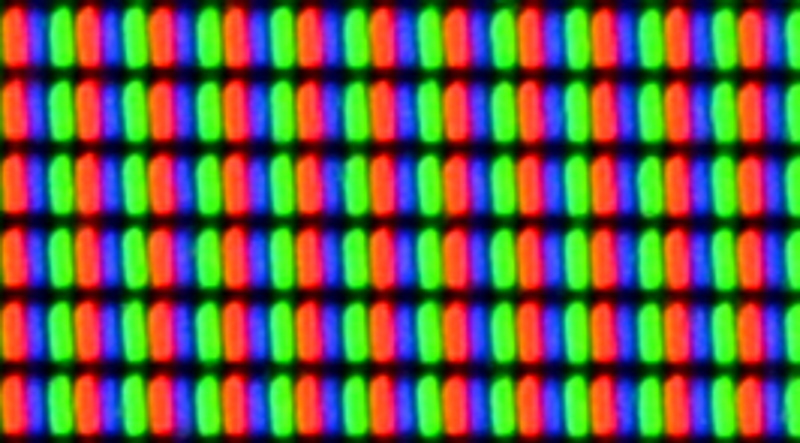
\includegraphics[width=80truemm]{slike/09_LCD.jpg}
\caption{Na močno povečani fotografiji računalniškega tekočekristalnega zaslona se 
jasno vidi, da je vsak piksel sestavljen iz treh delov: rdečega, modrega in zelenega.}
\label{fig:LCD}
\end{figure}
\begin{remark}
Tekočekristalni zasloni, ki jih uporabljamo danes, so precej bolj zapleteni.
Najpreprostejši so črno-beli prikazovalniki, ki delujejo z odbito svetlobo (npr. 
v žepnih računalih), zato imajo za analizatorjem odbojno površino. Večina 
sodobnih prikazovalnikov (npr. računalniški ali telefonski zasloni) ima svoj izvor svetlobe, 
praviloma so to LED ali fluorescenčna svetila.
Barve dosežemo z barvnimi filtri (rdečim, modrim in zelenim, slika~\ref{fig:LCD}) na vsakem 
slikovnem elementu (pikslu) posebej, krmiljenje pikslov pa s tankoplastnimi 
tranzistorji (TFT - {\it Thin Film Transistors}). Večina
sodobnejših zaslonov ima tekoče kristale urejene planarno in v njih poteka
preklapljanje v ravnini (IPS - {\it In-Plane Switching}), lahko so molekule
urejene vertikalno in jih s poljem nagibamo (VA - {\it Vertical Alignment}), tekočekristalne 
zaslone lahko z dodatnimi plastmi naredimo tudi občutljive na dotik.
\end{remark}
\vglue-3truecm
\section{*Račun prehoda svetlobe skozi zasukan nematik}
\index{Tekoči kristali!zasukan nematik}
Pokazati moramo še, da polarizacija svetlobe pri prehodu skozi zasukan nematik 
približno sledi zasuku optične osi.\footnote{Glej npr. P. G. de Gennes in J. Prost, 
{\it The Physics of Liquid Crystals}, Oxford University Press (1995).}\index{Dvolomnost!enoosne snovi}
Vzemimo vzorec, kakršen je na sliki~\ref{LCD1}\,a in ga obravnavajmo
kot lokalno optično enoosno snov. Pri $z=0$ naj bo optična
os v smeri $x$, ko se premikamo vzdolž osi $z$, naj se optična os suče
v ravnini $xy$. Kot med optično osjo in osjo $x$ tako zapišemo 
\begin{equation}
\varphi=qz.
\label{7.58}
\end{equation}
Zanimajmo se le za širjenje svetlobe v smeri $z$. 
Tedaj potrebujemo le del dielektričnega
tenzorja v $xy$ ravnini.\footnote{Podobno opišemo holesterični tekoči kristal, v
katerem so molekule kiralne in se $\mathbf{n}$ spontano suče okoli
smeri, pravokotne na $\mathbf{n}$.} 

\begin{definition}
Pokaži, da se dielektrični tenzor v zasukani nematični plasti zapiše kot\index{Dielektričnost}
\begin{equation}
\varepsilon (z)=\left[\begin{array}{cc}
\bar{\varepsilon}+\frac{1}{2}\varepsilon_{a}\cos(2qz) & \frac{1}{2}\varepsilon_{a}\sin(2qz)\\
\frac{1}{2}\varepsilon_{a}\sin(2qz) & \bar{\varepsilon}-\frac{1}{2}\varepsilon_{a}\cos(2qz)
\end{array}\right],
\label{7.59}
\end{equation}
kjer  je $z$ razdalja od plasti, v kateri je direktor
obrnjen v smeri $x$, in povprečna vrednost $\bar{\varepsilon}$ 
\begin{equation}
\bar{\varepsilon}=(\varepsilon_{\parallel}+\varepsilon_{\perp})/2.
\label{7.60}
\end{equation}
Namig: Uporabi rotacijsko matriko $A(\varphi)$ in izračunaj  $\varepsilon (z) = A(\varphi) \cdot 
\tilde{\varepsilon} \cdot A(\varphi)^\mathrm{T}$.
\end{definition}

Iz Maxwellovih enačb~(enačbe~\ref{eq:Maxwell1}--\ref{eq:Maxwell4}) 
hitro uvidimo, da je valovna enačba\index{Valovna enačba}
za valovanje s krožno frekvenco $\omega$ v našem primeru oblike
\begin{equation}
\frac{d^{2}\mathbf{E}}{dz^{2}}+\frac{\omega^{2}}{c^{2}} \epsilon
(z)\mathbf{E}=0
\label{7.61}
\end{equation}
ali po komponentah, upoštevajoč tenzor dielektričnosti~(enačba~\ref{7.59})
\begin{equation}
\frac{d^{2}E_{x}}{dz^{2}} + 
(\beta^{2}+\alpha^{2}\cos(2qz))E_{x}+\alpha^{2}E_{y}\sin(2qz) = 0
\label{7.62a}
\end{equation}
in 
\begin{equation}
\frac{d^{2}E_{y}}{dz^{2}} +
\alpha^{2}E_{x}\sin(2qz)+(\beta^{2}-\alpha^{2}\cos(2qz))E_{y} = 0,
\label{7.62b}
\end{equation}
kjer je $\alpha^{2}=\epsilon_{a}\omega^{2}/(2c^{2})$ in 
$\beta^{2}=\bar{\epsilon}\omega^{2}/c^{2}$. S tem smo dobili sistem
dveh sklopljenih diferencialnih enačb, ki ga lahko rešimo.
\begin{remark}
Opis potovanja svetlobe skozi zasukan nematik je lepa ilustracija uporabe 
Blochovega teorema, ki ga sicer poznamo iz fizike trdne snovi za 
reševanje Schr\"odingerjeve enačbe za delec v periodičnem potencialu. Teorem pravi, 
da lastne rešitve zapišemo kot produkt ravnega vala in funkcije, ki ima enako 
periodo kot potencial.\index{Blochov teorem}\footnote{Glej npr. N. W. Ashcroft in 
N. D. Mermin, {\it Solid State Physics}, Harcourt College
Publishers (1976).}
\end{remark}

Za reševanje je ugodno vpeljati krožni polarizaciji 
$E_{+}=E_{x}+iE_{y}$ in $E_{-}=E_{x}-iE_{y}$.
Enačbi~(\ref{7.62a}) in (\ref{7.62b}) prepišemo v
\begin{equation}
-\frac{d^{2}E_{+}}{dz^{2}}=\beta^{2}E_{+}+\alpha^{2}E_{-}e^{2iqz}
\label{lcm1}
\end{equation}
in 
\begin{equation}
-\frac{d^{2}E_{-}}{dz^{2}}=\alpha^{2}E_{+}e^{-2iqz}+\beta^{2}E_{-}.
\label{lcm2}
\end{equation}

Lastne rešitve poiščemo v obliki 
\begin{equation}
E_{+}  =  Ae^{i(k+q)z} 
\qquad
\mathrm{in}
\qquad
E_{-}  =  Be^{i(k-q)z}.
\label{7.65}
\end{equation}
Nastavek reši sistem enačb~(\ref{lcm1}) in (\ref{lcm2}) 
natanko takrat, kadar $A$ in $B$ rešita sistem homogenih linearnih enačb 
\begin{equation}
\left((k+q)^{2}-\beta^{2}\right)A-\alpha^{2}B  =  0 \qquad \mathrm{in} \qquad 
-\alpha^{2}A+\left((k-q)^{2}-\beta^{2}\right)B  =  0.
\label{7.66d}
\end{equation}
 Sistem je netrivialno rešljiv, če je determinanta koeficientov enaka
nič
\begin{equation}
\left(k^{2}+q^{2}-\beta^{2}\right)^{2}-4k^{2}q^{2}-\alpha^{4}=0.
\label{7.66}
\end{equation}
Spomnimo se, da sta $\beta$ in $\alpha$ sorazmerna z $\omega$,
zato dobljena enačba predstavlja disperzijsko relacijo -- zvezo med 
$\omega$ in $k$ -- za svetlobo v zasukanem sredstvu
\begin{equation}
\left(k^{2}+q^{2}-\frac{\bar{\epsilon}\omega^{2}}{c^{2}}\right)^{2}-
4k^{2}q^{2}- \frac{\epsilon_{a}^2\omega^{4}}{4c^{4}}
=0.
\label{7.66a}
\end{equation}

Da dobimo disperzijsko odvisnost, moramo rešiti kvadratno enačbo (enačba~\ref{7.66a}). 
Vendar za razlago delovanja zasukane nematične celice zadošča približek 
$q\ll\alpha, \beta$, saj je perioda sukanja optične osi
velika v primerjavi z valovno dolžino svetlobe. Tedaj lahko $q$ v disperzijski
zvezi (enačba~\ref{7.66}) zanemarimo in velja
\begin{equation}
k^{2}=
\begin{cases}
\beta^{2}+\alpha^{2}=\frac{\omega^{2}}{c^{2}}\epsilon_{\parallel}\\
\beta^{2}-\alpha^{2}=\frac{\omega^{2}}{c^{2}}\epsilon_{\bot}.
\end{cases}
\label{7.67}
\end{equation}
Ti dve vrednosti ustrezata velikosti valovnega vektorja za izredni
in redni val v navadnem enoosnem kristalu. Vstavimo ju v enačbi~(\ref{7.65})
in za polarizaciji lastnih valov dobimo $B=\pm A$.
Izračunajmo še obe kartezični komponenti električnega polja za prvo rešitev ($A=B$)
\begin{align}
E_{x} &=  \frac{1}{2}(E_{+}+E_{-})  =  \frac{1}{2}Ae^{ikz}(e^{iqz}+e^{-iqz})  =  Ae^{ikz}\cos qz\\
E_{y} & = \frac{1}{2i}(E_{+}-E_{-})  =  \frac{1}{2i}Ae^{ikz}(e^{iqz}-e^{-iqz})  =  Ae^{ikz}\sin qz.
\label{7.68}
\end{align}
Zasuk polarizacije torej sledi zasuku optične osi. Druga rešitev ($A=-B$) da val,
ki je polariziran pravokotno na lokalno optično os in se prav tako
suče z njo. Pri tem se prvi val širi kot izredni val s fazno hitrostjo $c/n_{e}$ in  
drugi kot redni val s $c/n_{o}$. Če na zasukano
nematično celico vpada svetloba, ki je polarizirana ali vzporedno z 
optično osjo ob meji ali pravokotno nanjo, izstopa iz celice svetloba, katere 
polarizacija je zasukana za enak kot, kot je zasukana optična os. 
V primeru, da vpadna polarizacija ne sovpada z eno od
lastnih osi, jo razstavimo na lastni in po prehodu skozi
vzorec zopet sestavimo, s čemer seveda na splošno nastane eliptična
polarizacija.

\begin{remark}
Disperzijsko zvezo (enačba~\ref{7.66a}) 
lahko rešimo (slika~\ref{gap}). Pri izbrani vrednosti $\alpha$ 
obstajajo pri vseh frekvencah, razen v ozkem območju -- rečemo mu frekvenčna reža --
štiri realne rešitve za $k$, po dve za valovanji v pozitivni in v negativni smeri.
V območju reže je en par rešitev imaginaren. Vsaki vrednosti $k$
pripada neko razmerje amplitud $A$ in $B$, ki ga izračunamo
iz enačb~(\ref{7.66d}) in ki določa polarizacijo lastnega vala. Polarizacije
lastnih valov so na splošno eliptične in pri dani frekvenci med
seboj niso pravokotne, saj zapisani sistem enačb ne predstavlja čisto 
navadnega problema lastnih vektorjev simetrične matrike. 
V območju frekvenčne reže le en par rešitev predstavlja
potujoč val, drug pa polje, ki eksponentno pojema v sredstvo. Zato
se svetloba s frekvenco v reži in z ustrezno polarizacijo totalno odbije. Pojav v zasukanih
nematskih celicah ni opazen, saj je tam $q \ll \alpha$. Če pa je perioda vijačnice
primerljiva z valovno dolžino svetlobe, kot na primer v holesteričnih
tekočih kristalih, pride do značilnega obarvanega videza. Pojav
je povsem analogen Braggovemu odboju na kristalih.\index{Tekoči kristali!holesterik}\index{Braggov odboj}
\begin{figure}[h]
\centering
\def\svgwidth{80truemm} 
\input{slike/09_gap.pdf_tex}
\caption{Rešitve disperzijske zveze (enačba~\ref{7.66}) v zasukanem nematiku
ali holesteriku pri danem $\alpha$. Razen v frekvenčni reži (modra pasova) obstajajo štiri 
rešitve pri vsaki frekvenci.}
\label{gap}
\end{figure}
\end{remark}

\section{Račun preklopa v tekočem kristalu -- Frederiksov prehod}
Ob opisu tekočekristalnih prikazovalnikov smo omenili, da lahko z dovolj velikim 
zunanjim električnim poljem molekule tekočega kristala, razen tik ob urejevalni površini,
obrnemo v smeri polja. Izračunajmo jakost polja, ki je potrebna za ta zasuk. 
\index{Frederiksov prehod}

Energija nematičnega tekočega kristala je najnižja, kadar je direktor $\mathbf{n}$
povsod obrnjen v isto smer. Povečanje energije zaradi krajevne odvisnosti $\mathbf{n}$
zapišemo z orientacijsko elastično energijo oziroma Frankovo prosto 
energijo\footnote{Angleški fizik Sir Frederick Charles Frank, 1911--1998.}
\index{Frankova prosta energija}
\boxeq{7.70}{
F_{e}=\frac{1}{2}\int\left\{ K_{1}(\nabla\cdot\mathbf{n})^{2}+K_{2}
\left(\mathbf{n}\cdot(\nabla\times\mathbf{n})\right)^{2}+K_{3}
\left(\mathbf{n}\times(\nabla\times\mathbf{n})\right)^{2}\right\} dV.
}
Pri tem so $K_{1}$, $K_{2}$ in $K_{3}$ tri Frankove elastične
konstante, ki so odvisne od snovi in tudi od temperature. 
Prvi člen predstavlja povečanje energije zaradi deformacije v obliki 
pahljače, drugi zaradi zasuka in tretji zaradi upogiba (slika~\ref{s7.20}).\footnote{F. C.
Frank, Discuss. Faraday Soc. $\mathbf{25}$, 19 (1958).}
\begin{figure}[h]
\centering
\def\svgwidth{140truemm} 
\input{slike/09_KKK.pdf_tex}
\caption{Trije načini deformacije ureditve molekul tekočega kristala so pahljačasta deformacija,
zasuk in upogib.}
\label{s7.20}
\end{figure}

V zunanjem električnem polju se energija tekočega kristala dodatno spremeni. 
Navadno je neodvisna količina jakost električnega polja, saj je polje posledica
zunanje napetosti na elektrodah. Ustrezni člen v prosti energiji je tedaj 
(enačbi~\ref{lcwe} in~\ref{7.56a})
\begin{equation}
F_{el} = -\int \frac{1}{2} \mathbf{D}\cdot\mathbf{E}\, dV= -\frac{1}{2} \int
\left( \varepsilon_0 \varepsilon_\bot \mathbf{E}\cdot\mathbf{E} + 
\varepsilon_{0}\varepsilon_{a}(\mathbf{E}\cdot\mathbf{n})^{2}\right)dV = F_0 + F_{el,a}.
\end{equation}
Pri tem $F_{0}$ predstavlja del proste energije, ki je neodvisen od $\mathbf{n}$ in 
zato ni pomemben pri izračunu preklopa. Prosta energija
nematičnega tekočega kristala v električnem polju je tako 
\begin{equation}
F=F_e + F_{el} = F_0 + F_e + F_{el,a} = F_{0}+F_{e}-\int \frac{1}{2}\varepsilon_{0}\varepsilon_{a}
(\mathbf{E}\cdot \mathbf{n})^{2}dV.
\label{7.72}
\end{equation}
Tekoči kristal je v ravnovesju, ko je prosta energija najmanjša. Kadar je
$\epsilon_{a}>0$, se zato skuša $\mathbf{n}$ postaviti vzporedno s
poljem, vendar popoln zasuk onemogoča mejna urejevalna plast. 
Da lahko z minimizacijo $F$ izrazimo $\mathbf{n}(\mathbf{r})$, moramo
torej poznati še robne pogoje.

Naj bo nematični tekoči kristal med dvema vzporednima
steklenima ploščama, med katerima je razmik $d$. Na obeh ploščah naj bo $\mathbf{n}$ vzporeden
s površino in obrnjen v isto smer, tako da je brez zunanjega 
polja $\mathbf{n}$ povsod enako usmerjen. Naj bo to smer $x$.
Na stekleni plošči dodamo elektrodi, ki ustvarjata polje pravokotno na 
prvotno smer direktorja, naj bo to smer $z$.
Ko priključimo polje, je energijsko ugodnejše, da
se molekule vsaj delno zasučejo v smer polja. Ta zasuk opišemo s
komponento vektorja $\mathbf{n}$ v smeri $z$
\begin{equation}
\mathbf{n}(z)=(n_{x}(z),0,n_{z}(z)).
\label{7.73}
\end{equation}
Robni pogoj, kateremu mora direktor zadostiti,
je $n_{z}(0)=n_{z}(d)=0$. Približno rešitev zato iščemo z nastavkom 
\begin{equation}
n_{z}(z)=a\sin (qz), \qquad q=\frac{\pi}{d},
\label{7.74}
\end{equation}
ki ni nič drugega kot prvi člen razvoja prave rešitve v Fourierevo vrsto.
Ker je direktor enotski vektor, velja
\begin{equation}
n_x = \sqrt{1-a^2\sin^2(qz)} \approx 1 - \frac{a^2}{2}\sin^2(qz).
\end{equation}
Vzdolž smeri $x$ in $y$ se direktor ne spreminja, zato velja
\begin{equation}
\nabla\times\mathbf{n}=\left(0,\frac{dn_{x}}{dz},0\right)
\label{7.75}
\end{equation}
 in 
\begin{equation}
\mathbf{n}\times(\nabla\times\mathbf{n})=\left(-n_{z}\frac{dn_{x}}{dz},0,
n_{x}\frac{dn_{x}}{dz}\right).
\label{7.76}
\end{equation}
Prosta energija na enoto površine je tako do konstante
\begin{align}
F_S & =  \frac{1}{2}\int\left(K_{1}\left(\frac{dn_{z}}{dz}\right)^{2}+K_{3}(n_x^2+n_{z}^{2})
\left(\frac{dn_{x}}{dz}\right)^{2}-
\epsilon_{0}\epsilon_{a}(n_{z}E)^{2}\right)dz=\nonumber \\
 & =  \frac{1}{2}\int_{0}^{d}
 \left(K_{1}q^{2}a^{2}\cos^{2}(qz)+K_{3}q^{2}a^{4}\sin^{2}(qz)\cos^2(qz)-
 \epsilon_{0}\epsilon_{a}E^2a^{2}\sin^{2}(qz)\right)dz=\nonumber \\
 & =  \frac{d}{4}\left( K_{1}q^{2}a^2+\frac{1}{4}K_{3}q^{2}a^4-\epsilon_{0}\epsilon_{a}E^2a^2\right).
\end{align}
V našem primeru smo integral lahko izračunali, saj smo uporabili nastavek (enačba~\ref{7.74}).
Sicer bi morali uporabiti Euler-Lagrangeevo metodo za minimizacijo proste energije, ki 
jo poznamo iz variacijskega računa.

Zdaj lahko poiščemo amplitudo deformacije $a$, pri kateri je prosta energija
najmanjša in odvod $dF_S/da=0$. Tedaj mora biti $a$ rešitev enačbe 
\begin{equation}
2(K_{1}q^{2}-\epsilon_{0}\epsilon_{a}E^2)a+K_{3}q^{2}a^{3}=0.
\label{7.78}
\end{equation}
 Rešitvi sta 
\begin{equation}
a=0
\end{equation}
in
\begin{equation}
a^{2}=2\frac{\epsilon_{0}\epsilon_{a}E^2-K_{1}q^{2}}{K_{3}q^{2}}.
\label{7.79}
\end{equation}
 Pri majhnih poljih, ko je $\epsilon_{0}\epsilon_{a}E^2<K_{1}q^{2}$,
je fizikalno smiselna le prva rešitev, ki predstavlja vzorec brez deformacije. Pri 
velikih poljih postane stabilna druga rešitev. Takrat deformacija
v sredini plasti hitro naraste, tako da se $\mathbf{n}$ postavi skoraj
popolnoma v smer zunanjega polja.Tedaj naša rešitev seveda ni dobra,
saj smo pri računu privzeli, da je $n_{z}\ll1$. Prehodu iz nedeformiranega
stanja v deformirano stanje pravimo  Frederiksov prehod\footnote{Ruski fizik
Vsevolod Konstantinovič Frederiks, tudi Fr\'{e}edericksz, 1885--1944.}.\footnote{
V. Frederiks in V. Zolina, Trans. Faraday Soc. $\mathbf{29}$, 919 (1933).}  Na njem
temelji preklapljanje optičnih prikazovalnikov na nematične tekoče kristale.

Izračunajmo še kritično jakost električnega polja, pri kateri pride do prehoda v deformirano fazo.
To se zgodi pri 
\begin{equation}
\epsilon_{0}\epsilon_{a}E_c^2-K_{1}q^{2} = 0
\end{equation}
oziroma
\boxeq{FreeE}{
E_c = \frac{\pi}{d}\sqrt{\frac{K_1}{\varepsilon_0\varepsilon_a}}.
}
V tipičnem tekočekristalnem prikazovalniku je napetost, potrebna za prehod, $U = E_cd \sim 3~\si{\volt}$. 
\index{Tekočekristalni prikazovalnik}

Poglejmo še, kako narašča amplituda deformacije v bližini prehoda. Iz enačbe~(\ref{7.79})
sledi 
\begin{equation}
a = \sqrt{\frac{2 \varepsilon_0 \varepsilon_a}{K_3 q^2 }(E^2-E_c^2)}.
\end{equation}
Pogosto naredimo približek enakih konstant, kjer privzamemo, da so vse Frankove 
elastične konstante enake vrednosti. V tem približku je 
\begin{equation}
a \approx \sqrt{\frac{2(E^2-E_c^2)}{E_c^2}}
\end{equation}
in amplituda korensko narašča s naraščajočim poljem (slika~\ref{Fred}). Tak prehod je
fazni prehod drugega reda, saj količina, ki opisuje prehod (amplituda deformacije $a$)
zvezno preide iz vrednosti $a=0$ v končno vrednost. 
\begin{figure}[h]
\centering
\def\svgwidth{70truemm} 
\input{slike/09_Fred.pdf_tex}
\caption{Kvalitativno obnašanje amplitude deformacije $a$ ob Frederiksovem prehodu. Pri poljih, 
manjših od kritičnega, so molekule tekočega kristala urejene, nad kritičnim poljem
pa se ureditev deformira.}
\label{Fred}
\end{figure}

\begin{definition}
Izračunaj Frederiksov prehod v zasukani nematični celici (kot zasuka med zgornjo in spodnjo 
mejno ploskvijo naj bo $\pi/2$) in pokaži, da je kritično polje za prehod enako
\begin{equation}
E_c =  \frac{\pi}{d}\sqrt{\frac{K_1}{\varepsilon_0\varepsilon_a}}
\sqrt{1 + \frac{K_3-2K_2}{4K_1}}.
\end{equation}
Namig: uporabi nastavek $\varphi = z \pi/2d$ in $\vartheta = a \sin(\pi z/d)$. 
\end{definition}
